\chapter{Introduction}

%\section{Importance}

Psychiatric and substance abuse disorders account for 7.1\% of disease burden as measured by disability-adjusted life years\cite{murray2015global}.   A range of environmental and genetic factors are known to be implicated in their development. Of the genetic factors, most encode molecules that are found in the neuronal synapse, a structure that is responsible for the exchange and processing of information between nerve cells\cite{grant2012synaptopathies}.

\section{The synaptic proteome}

This thesis is about synapses and cognition, specifically how the complicated interactions of the proteins making up synapses may affect the efficiency of cognition in man and model animals. 

The synapse is a complex system composed of thousands of proteins that form higher order structures (the synaptic proteome)\cite{grant2012synaptopathies}. There have been great advances in the understanding of the molecular mechanisms of synaptic function in the last 20 years\cite{grant2018synaptomic}. The synaptic proteins form a complex system and to understand their role in health and disease it is necessary to understand how it functions as a system.  One important way of understanding complex systems is as a network where nodes, in this case proteins, are joined by edges if they interact. 



This thesis will investigate if a network analysis of the synaptic proteome is useful in understanding the molecular basis of cognition. In particular it will see whether there is evidence of an effect of the structure of synaptic protein interactions on animal models of cognition or human population studies of cognitive ability. It will test the hypothesis that genes encoding proteins that are more important to the network are over represented in animal models of cognition or in human population studies of intelligence or educational attainment. It will also assess whether particular structures found in the network topology have an effect on human or animal cognitive function. Before turning to the network structure of the synapse and population studies of cognition it is necessary to introduce the structure and function of the excitatory synapses that will be discussed in the coming chapters. 

\subsection{Synapse introduction}
A nerve cell is composed of a number of dendrites that receive incoming signals, a cell body or soma and an axon that transmits outgoing signals (figure~\ref{fig:soma and dendrites}). Between the axon and the dendrite are synapses (see figure~\ref{fig:synapse}).Synapses are junctions where information transfer occurs between nerve cells and are the most abundant structure in the brain \cite{grant2012synaptopathies}.

% In addition, although less marked in recent years, genetic approaches to cognitive ability remain highly controversial. In describing a computational systems biology approach to cognition, although it may appear clear from this review, it is important to avoid the implication that this implies a computatio\cite{deary2009genetic}. In addition, although less marked in recent years, genetic approaches to cognitive ability remain highly controversial. In describing a computational systems biology approach to cognition, although it may appear clear from this review, it is important to avoid the implication that this implies a computational model of mind or of cognitive abilities. 
% nal model of mind or of cognitive abilities. 


\begin{figure}
    \centering
    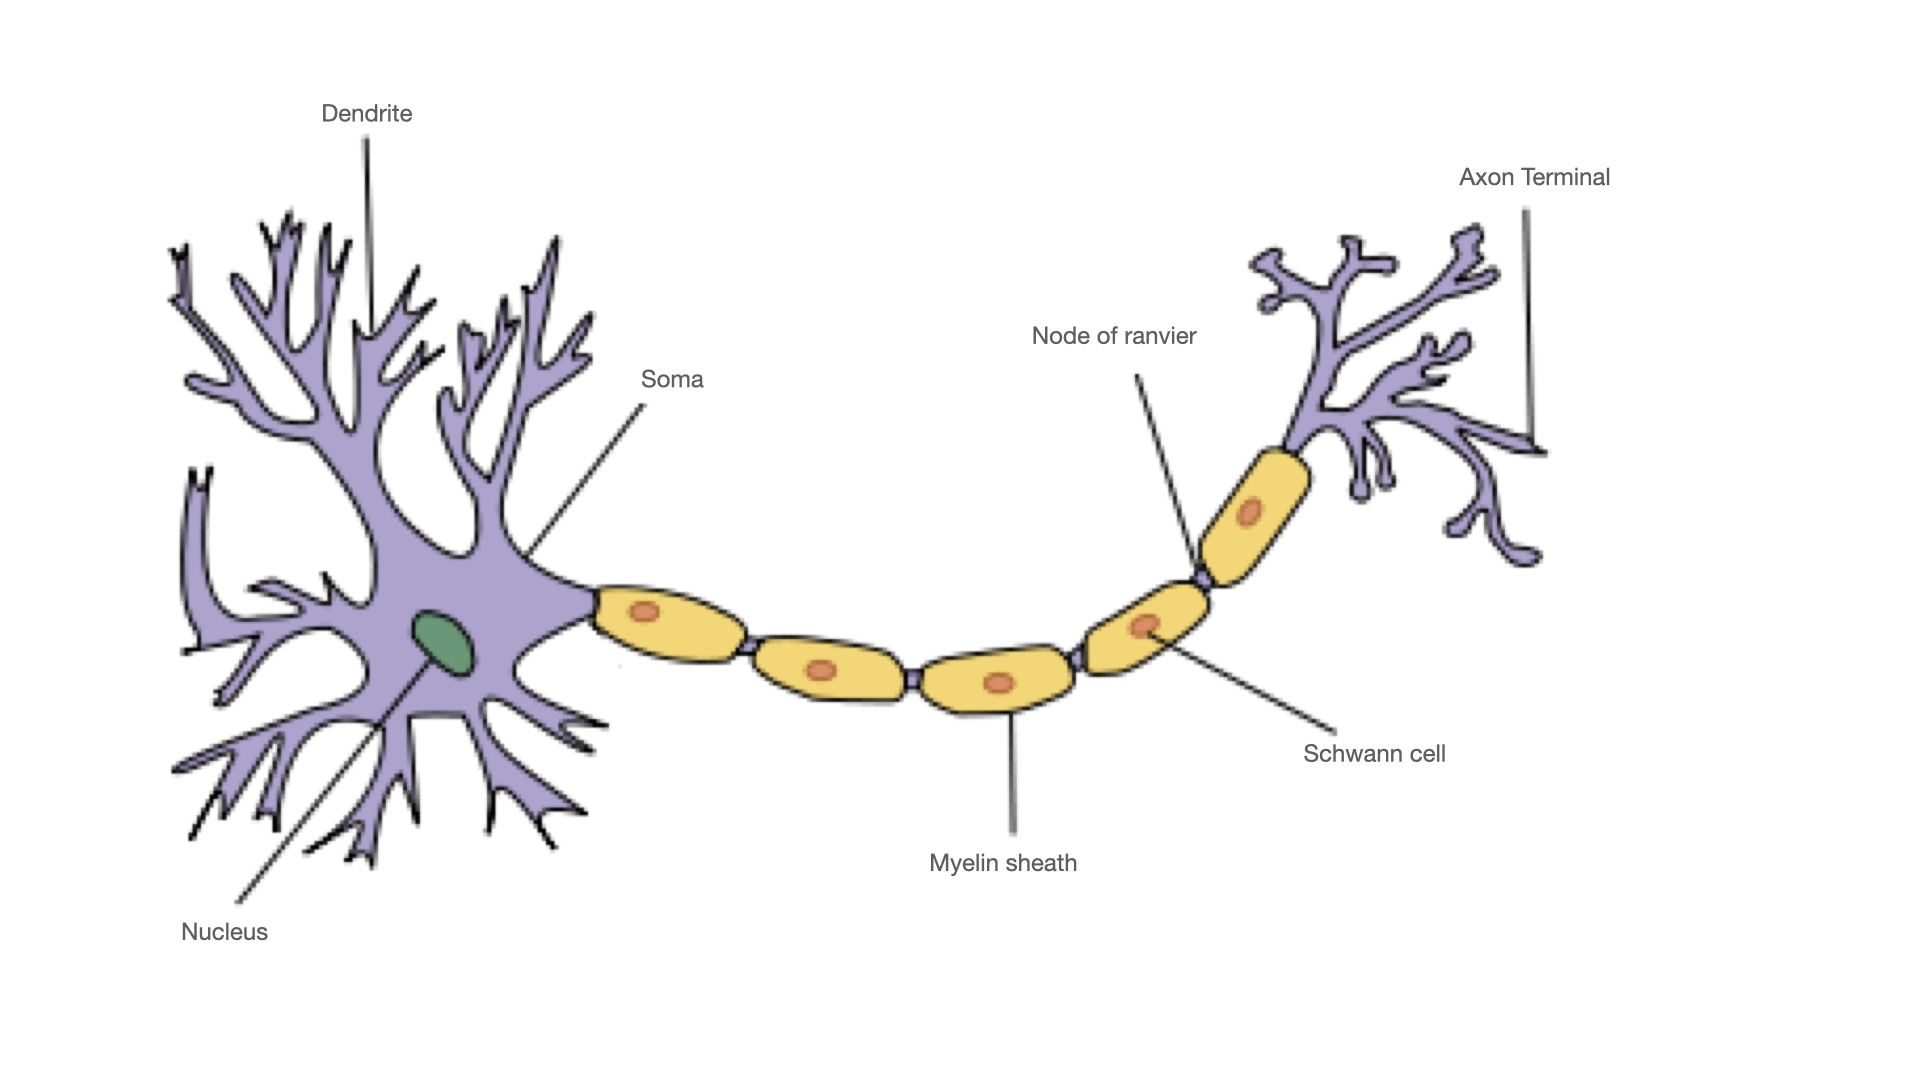
\includegraphics[width=0.9\textwidth]{images/nerve_cell001.jpeg}
    \caption{Soma and dendrites}
    \label{fig:soma and dendrites}
\end{figure}

Each nerve cell has one outgoing axon but a cortical neuron receives input from around 100,000 synapses, although only around 50 are active at any one time\cite{lisman2017glutamatergic}\footnote{number has varied see also \cite{laughlin2003communication} which has 10,000}. 
Although synaptic numbers vary over time, the number of synapses in the human neo-cortex has been estimated to be $1.5 \times 10^{14}$ (0.15 quadrillion)\cite{pakkenberg2003aging}. A synapse connects a presynaptic neuron and a postsynaptic cell across the synaptic cleft \cite{sudhof2012presynaptic}. The synapse is made up of proteins that self organise into macro-molecular machines that are responsible for signal transduction and processing\cite{frank2016nmda}.  The nerve cell integrates incoming information from the dendrites into a binary response at the axon\cite{lassek2015synaptic},\cite{pocklington2006proteomes}.

 The majority of synapses in the brain belong either to the excitatory glutamate system or the inhibitory gamma-aminobutyric acid (GABA) system. The most common type of synapse and neurotransmitter are the glutamatergic excitatory transmitters which comprise the main information processing system in the brain \cite{stewart2014structure},\cite{niciu2012overview} \footnote{was a todo: previous ref stewart2014structure changes second ref ok}. Glutamate is also a precursor for GABA. 

The term synapse, from the Greek ``to clasp together" was coined by Sherrington in 1897 writing in Foster’s textbook of physiology \cite{foster1895text}. Since Cajal showed that there was a gap between nerve cells the accepted model of the nervous system has been of a structure composed of nerve cells built into higher order circuits\cite{ramon1911histologie},\cite{grant2018synapse} rather than a reticulum or syncytium\footnote{although some still do see \cite{bacsar2016clair}}. Cognitive complexity was thought to arise from an increasing number of connections (the neuronal hypothesis)\cite{grant2018synaptomic}.
%\todo{ ? expand this section}
%\todo{need ref for cognitive complexity}
\subsection{Molecular genetic revolution}
\label{sec:molecular genetic revolution}
 The neuronal hypothesis holds that the brain's functional unit is the neural circuit and that brain complexity arises from the pattern of nerve cell and circuit connections\cite{grant2018synaptomic}. Quite recently the molecular interactions of the synapse were believed to be relatively simple with a small number of proteins sufficient for signal transfer and the control of synaptic connection strength \cite{grant2019synapse}, \cite{lisman1994cam}. This hypothesis is not unreasonable, simple models of neurons can carry out complex calculations requiring only weights at their connections analogous to connection strength at synapses\cite{hinton2007learning}. Synaptic function as signal transmission and modulation of connection strength concurred with the model of learning by increasing synaptic strength formalised by Hebb \cite{hebb1949organization_check}.
 
 Direct molecular interrogation of synaptic proteins became possible with mouse models in 1992 allowing the identification of synaptic proteins and the study of their function using knockdowns  \cite{grant1992impaired},\cite{silva1992impaired}. Further advances in molecular genetics revealed the complexity of the synaptic proteome. In 2000 Husi et al. \cite{husi2000proteomic} identified 77 proteins in the N-methyl-D-aspartate (NMDA) receptor complex (NRC). Over the next 5 years many more synaptic proteins were identified. In 2006 an analysis considered the network of 186 proteins in the NRC/Membrane Associated Guanylate Kinase (MAGUK) associated signalling complex (NRC/MASC) \cite{pocklington2006proteomes}. The number of known proteins in the post synaptic proteome rose to 1,124 by 2006\cite{collins2006molecular}.
 
The number of proteins and the complexity of their interactions exceeded what might be expected to be necessary to simply maintain connection strength 
%\todo{have we introduced connection weight}
and led to the recognition that the proteome was vitally involved in signal processing and computation as well as signal transduction\cite{grant2018synaptomic}.  Over 3,000 proteins have now been identified in proteomic studies of the post synaptic density (PSD), although this number appears to be reaching a plateau\cite{heil2018systems}. 
%\todo{query move this bit}
The proteins that form the structure of the post synaptic area are modular and form higher order complexes whose structure is related to their function\cite{pocklington2006proteomes},\cite{zhu2016mechanistic},\cite{frank2016nmda}. To understand the synapse we must try to understand the complexity of this system.

\begin{figure}
    \centering
    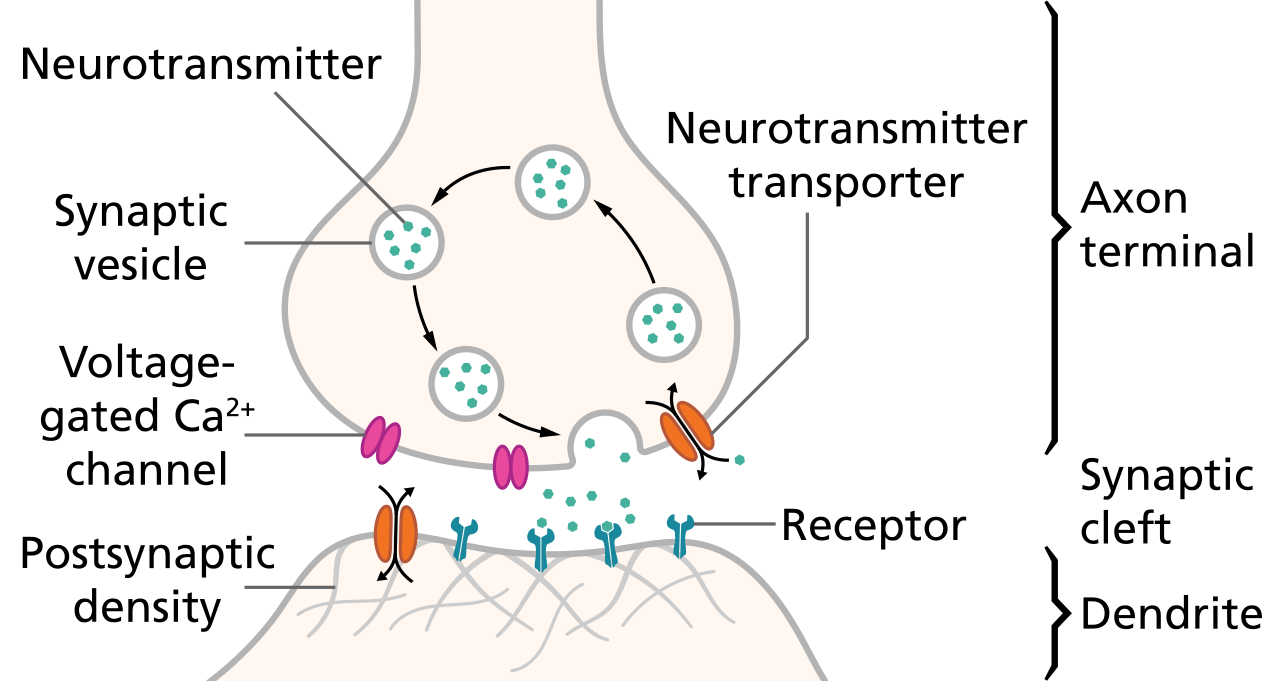
\includegraphics[width=0.9\textwidth]{images/SynapseSchematic_en.png}
    \caption[Schemtatic representation of synapse]{Schematic representation of synapse showing presynaptic area (labelled axon terminal) containing vesicles rich in neurotransmitters and post synaptic density.  Picture credit Thomas Splettestoesser Creative Commons \url{https://commons.wikimedia.org/wiki/User:Splette}}
    \label{fig:synapse}
\end{figure}





\subsubsection{High level function of the synapse}

The synapse controls the strength of the connection between nerve cells. If the activation of one nerve cell repeatedly activates another their connection will strengthen over time (Hebbian learning)\cite{hebb1949organization_check}. Hebb's rule \cite{hebb1949organization_check} requires the arrival of a signal at the presynaptic terminal, and consequent postsynaptic depolarisation leading to a stronger synaptic connection.  As neural circuits determine behaviour, these repeated patterns of activation form a basis for learning.%\todo{this end of sentence new review}.

The discovery of long term potentiation (LTP) by Bliss and Lomo \cite{bliss1973long} ultimately led to the discovery of the importance of glutamate transmission in LTP and that disruption of synaptic proteins reduces LTP and learning. Hebb posited a model where the connection strength between two neurons depends on how often they are activated together.  Both short term potentiation and long term potentiation are involved in adaptive neural information processing by controlling the strength of the connections between neurons\cite{xiao2013adaptive}.

\section{Synapse structure}
\label{sec:Synaptic structure}
The synapse is composed of a presynaptic area filled with neurotransmitter vesicles and a postsynaptic area containing neurotransmitter receptors and structural proteins separated by a gap. Nerve signals arrive at the presynaptic area, cause or inhibit the release of neurotransmitters from synaptic vesicles which diffuse across the cleft and are detected by postsynaptic receptors whose activation may lead to depolarisation of the cell axon. 

%
\subsection{Presynaptic area structure}
The presynaptic area is separated from the post synapse by the synaptic cleft \cite{rusakov2011shaping}, an area approximately 20nm in size \cite{zuber2005mammalian},%\todo{fix missing circumflex in the first name of zuber DONE} 
spanned by trans-synaptic adhesion molecules\cite{missler2012synaptic}.

 The presynaptic area contains neurotransmitters stored in vesicles docked and fused with the plasma membrane at a specialised active zone. This is an electron-dense area, parallel and juxtaposed to the plasma membrane\cite{schoch2006molecular},\cite{sudhof2012presynaptic}. Neurotransmitters are substances which, when they diffuse across the synaptic cleft, give rise to signal in the postsynaptic receptors. Active vesicles are docked at the edge of the membrane and released following calcium influx \cite{lassek2015synaptic}. After neurotransmitter release, the vesicle is recycled by endocytosis\cite{ashery2014molecular}. Short term changes in synaptic plasticity (short term potentiation) are mainly caused by changes in the probability of presynaptic vesicle release. In contrast, long term potentiation occurs mostly at the postsynaptic density.  A substantial amount of neural computation occurs in the presynaptic area and is dependent on synaptic proteins \cite{sudhof2012presynaptic}.
 
 
  A protein complex of 5 evolutionarily conserved proteins: RIM, Munc13, $\alpha$-liprin, RIM BP and ELKS \cite{sudhof2012presynaptic} primes the vesicles. Piccolo and Bassoon proteins are also associated with the active zone in vertebrates\cite{gundelfinger2016role}.  SNARE proteins facilitate vesicular fusion \cite{sudhof2012presynaptic}. Mitochondria \cite{lassek2014proteome} are an integral part of the presynaptic area and were noted in early electron microscopy  examinations \cite{gray1959electron}. The active zone is closely associated with a cytoskeletal matrix: the cytoskeletal matrix at the active zone (CAZ) \cite{schoch2006molecular}. Post synaptic activation results in CAZ clustering \cite{glebov2017nanoscale}. 
 
   In some nerve cells such as  photoreceptors, the active zone is ribbon-like and capable of prolonged discharge  \cite{ashery2014molecular}.  
 
 
The presynaptic area developed from vesicle transport systems in earlier organisms and has developed more recently than the postsynaptic density (PSD)\cite{emes2012evolution}.

 
\subsection{The postsynaptic area and postsynaptic density}
\label{sec:post synaptic area and post synaptic density}
The postsynaptic density is an electron-dense area parallel to the synaptic plasma membrane and extending $\approx$ 35nm deep to it \cite{harris2012ultrastructure}. Formed from structural proteins that bind to actin in dendritic spines and to the receptor complexes, it contains protein kinases, receptor molecules and protein scaffold complexes such as postsynaptic density protein 95 (PSD-95). There are slight differences in its composition between mouse and man \cite{bayes2012comparative}, but in general, its component structures are conserved in vertebrates. The components of the postsynaptic area arose in the earliest prokaryotes to detect changes in chemical gradients with movement and are the most ancient part of the synapse developmentally \cite{grant2018synapse}, \cite{emes2012evolution}. 

Neurotransmitter chemicals typically mediate signal transfer across the synaptic cleft although direct electrical transmission can occur across gap junctions in the retina and some locations in the central nervous system \cite{stewart2014structure}. The neurotransmitter receptors are bound to cytoskeletal proteins and modified by members of the membrane-associated guanylate kinase family (MAGUK) of proteins involved in synaptic plasticity \cite{zhu2016mechanistic}. Glutamate release occurs in areas closely aligned with glutamate receptors in the postsynaptic density (PSD) \cite{harris2012ultrastructure}.

 The receptors in the postsynaptic density show a geographical variation with the $\alpha$-amino-3-hydroxy-5-methyl-4-isoxazolepropionic acid  receptors (AMPAR) and N-methyl D aspartate (NMDA) receptors in close apposition to the presynaptic active zone and the metabotropic glutamate receptors (mGluR) in the perisynaptic zone\cite{scheefhals2018functional}.
 
 The ionotropic receptors have the fastest signalling characteristics and include NMDAR, AMPAR  and Kainate receptors (KAR) named after the particular agonists found to provoke them\cite{nakanishi1992molecular},\cite{bettler1995ampa}. Kainate acid receptors have a metabotropic G protein-mediated element in their response that has been shown to mediate non NMDA LTP in the hippocampus of the rat \cite{petrovic2017metabotropic}. They are less involved in synaptic transmission \cite{contractor2011kainate} than the two pure ligand-gated ionotropic receptors NMDAR and AMPAR.
 \footnote{note to Douglas/self I am mentioning all this as group 5 has GRIA 1-4(AMPA), GRIK (Kainate) 1,2,3,5 and mGlu 2,3,7. 2 and 3 are Group II (activate K inhibit Ca and adenylyl cyvlase and pre and post synaptic, 7 is group7 and associated with presynaptic active zone}  
 The metabotropic glutamate receptor activates heterotrimeric G proteins and results in both signalling and recruitment of further ionotropic receptors to the postsynaptic area\cite{niswender2010metabotropic},\cite{pin2016organization}.  
 
Postsynaptic proteins show many remarkable features. They are relatively resistant to complete abolition of function \cite{keverne1997evaluation}, \cite{charlesworth2016canalization} and even in knockout animals, some signalling remains. In addition, the dysfunction of many disparate synaptic elements can result in common phenotypes, particularly neuropsychiatric phenotypes. A wide variety of mutations at different proteins and different loci within specific proteins can give rise to common disorders such as Autism Spectrum Disorder (ASD)\cite{toro2010key}. By contradistinction point mutations in crucial receptor proteins often give rise to severe phenotypes, as we shall see later, but also give rise to different phenotypes from mutations at different points in the protein (a case in point here being GRIN2A) \cite{endele2010mutations}. These features may in part be related to the organisation of the PSP into supercomplexes that inherit network based robustness\todo{tmp:cross ref} in addition to genetic robustness from paralogue expansion\cite{grant2016molecular}.



\subsection{Molecular function}
Calcium ion influx is necessary for depolarisation. Synaptotagmin acts as a calcium sensor and allows for the rapid fusion of synaptic vesicles with the cell membrane and release of neurotransmitters into the synaptic cleft\cite{martens2007synaptotagmin},  It is also necessary for learning in animals and long term potentiation and depression \cite{lisman2012mechanisms}.
\subsubsection{Neurotransmitter receptors}
\label{sec:Neurotransmitter receptors}
L glutamate, a small amino acid, is the dominant neurotransmitter at excitatory synapses within the brain \cite{niswender2010metabotropic}. Glutamate levels are controlled by the glutamate glutathione pathway and glutamate transporters\cite{sedlak2019glutathione}.

Fast excitatory neurotransmission is carried out at the ionotropic glutamate receptors AMPA and NMDA \cite{traynelis2010glutamate}. Ionotropic glutamate receptors consist of 4 sub-units spanning the extracellular membrane that form a central ion pore. AMPA and Kainate receptors are homo or heterotetrameric, but the NMDA receptor is obligatory heterotetrameric. The AMPA receptor is responsible for most of the fast excitatory transmission in the central nervous system \cite{henley2013ampa}. It is composed of four sub-units GRIA1-4 and is mainly permeable to sodium (Na$^+$) and potassium (K$^+$) ions. The glutamate receptor sub-units originate from 18 different gene protein products representing NMDA, AMPA, Kainate and delta groups \cite{traynelis2010glutamate}. The NMDA receptor is also composed of four subunits (a tetrameter)  but is permeable to calcium ions. AMPA and KAR are fast-acting, working in less than 1ms\cite{traynelis2010glutamate} wile NMDAR depolarise more slowly, in the 10ms range \cite{traynelis2010glutamate},\cite{nicoll2017brief}. 

Magnesium (Mg$^{2+}$) ions initially block NMDA receptor activity, and  AMPA receptor activation is required to displace the Mg$^{2+}$ ions. AMPA is intimately involved in long term potentiation. After Ca$^{2+}$ ion entry from the synaptic cleft, Calcium/calmodulin-dependent protein kinase II (CaMKII) is activated and leads to an increase in AMPA receptors at the postsynaptic membrane. Calcium can enter through NMDA receptors after unblocking of $Mg^{2+}$ ions, and its entry leads to activation of Calcium/Calmodulin dependent protein kinase. The kinase subsequently binds to NMDA receptors and phosphorylates sub-units of the AMPA type glutamate receptor.

Slow synaptic transmission, mediated by G protein second messengers, results from the action of metabotropic glutamate receptors (mGluR) \cite{niswender2010metabotropic} although mGluR signalling can also occur in time scales closer to ionotropic glutamate receptors (iGluR). There are eight mGluR subtypes. Metabotropic glutamate receptors are family C G-Protein-coupled receptors (GPCRs). Group 1 mGLU promote intracellular calcium release whereas group 2 are localised pre and postsynaptically, and group 3 are localised presynaptically \cite{niswender2010metabotropic}. 
\footnote{Note to self/Douglas and source code remove later - grm 2,3,7 in group 5 - 2 and 3 are in group 2, 7 along with 4,6,7,8 are om group 3, (grm 1 and 5 are group1), 1,2,3,5 and 7 are in the PSP, one is in 22 and 5 in group 32 - groups 20, 22 and 32 are quite closely related see \url{ source('~/RProjects/graph_groups/R/distribution_m_glu_glutamate.R')}Group II Metabotropic Glutamate Receptors Mediate Presynaptic Inhibition of Excitatory Transmission in Pyramidal Neurons of the Human Cerebral Cortex shows can be pre and postsynaptic } %However, there is also evidence for pre and postsynaptic action \todo{? more to discussion}
Metabotropic glutamate receptors exert their effect by increases in protein synthesis. Group II have been related to anxiety, schizophrenia and Alzheimer's disease\cite{swanson2005metabotropic}.


\subsubsection{Long term potentiation}
\label{sec:LismanLTP}
Periods of synaptic activity can increase the strength of synaptic connections by the process of long term potentiation (LTP).

Cajal first proposed that an increase in the strength of the connection between neural cells leads to learning in 1911 \cite{nicoll2017brief}. In Hebb's model synaptic modification occurs following coexistent pre and postsynaptic activation (two factors are required)\cite{hebb1949organization_check}. Later experiments showed that tetanic stimulation of rabbit hippocampal synapses increased the strength of subsequent responses\cite{bliss1973long}, and that NMDAR activity is necessary for LTP\cite{collingridge1983excitatory} but not for neurotransmission. 
 Interfering in the process of LTP in animal models leads to defects in memory and learning \cite{lisman2012mechanisms}).
LTP is a complex process with the modular organisation of 70-80nm modules of independently activating AMPA receptors being integral to the variety of potentiation responses\cite{lisman2017glutamatergic}. Six different forms of plasticity are observed in the synapse short term plasticity, long term plasticity, late long term plasticity, long term depression, distance-dependent scaling and homeostatic scaling \cite{lisman2017glutamatergic}. Short term potentiation (STP) results from weak stimuli and occurs early, and is a promising model of working memory as GluA1 knockdown animals have abnormal STP and working memory\cite{lisman2017glutamatergic}. Early LTP is likely mediated by phosphorylation of GluA1 by CaMKII. Late long term potentiation is associated with a change in the size of the PSD. LTP, by definition, begins 30 minutes after a tetanic stimulus. Late LTP is associated with more AMPAR signalling, protein synthesis\cite{park2018ampa} and an increase in quantal probability. This may require other factors such as dopamine in CA1 postulated as an indicator of salience or brain-derived neurotrophic factor (BDNF). For this reason (that three factors rather than two are required) the process has been referred to as NeoHebbian\cite{lisman2017glutamatergic}. The mechanisms of this late stage include increase in receptors from PSD 95 mediated CaMKII phosphorylation of Stargazin or SynGAP or activation of extracellular signal-regulated (ERK) kinase through SynGAP. Throughout all of this it is clear that memory and learning appear to intimately linked to  the combination and structure of synaptic proteins. \todo{tmp: that nonsense about memory molecule}

 
 
Computational models of the synapse have explain been developed that simulate these responses on the assumption that there are `hotspots' where there are either modules of AMPA receptor present or absent on vesicle release, and plasticity can occur with recruitment to silent hotspots\cite{lisman2017glutamatergic}.
 
 
\subsection{The synaptomic theory}

An alternative model of synaptic learning has been proposed where the complexity of the composition of the proteome is integral to learning\cite{grant2019synapse}. In this model, synaptic proteins form complexes and supercomplexes that are specifically attuned to different temporal neural signals and synaptic protein organisation acts as a `zip code' addressing different areas in the brain\cite{grant2018synaptomic}.

Evidence that is inconsistent with synaptic strength as the only mediator of learning\cite{grant2019synapse} include preservation of spatial learning after NMDA signalling and LTP have been blocked\cite{bannerman2014hippocampal} and mutations to PSD 95 leading to cognitive impairment but enhanced long term potentiation\cite{nithianantharajah2013synaptic}. It may be that the NMDA receptor both mediates learning and LTP\cite{grant2019synapse}. In this model too the modular structure of the proteome is closely related to its function in cognition. 

%  In contrast, Grant suggests a bottom-up synaptogenic model in which the synaptic protein composition acts as a zipcode which allows spatially distributed neurons to respond to particular patterns of receptor stimulation. In support of his arguments, he points out that the association of long term potentiation with learning remains controversial and it may be that the glutamate receptor (NMDA both subsume LTP and learning rather than affecting LTP which in turn causes learning. An example suggesting this is that mutations in PSD 95 give rise to cognitive impairments but increased long term potentiation.


\subsection{Role in disease}
 
Bayes et al.\cite{bayes2011characterization} identified, in human neocortical biopsies, 1,461 proteins in the human post synaptic density (hPSD) and 748 that were consistent across three replicates. Using the Online Mendelian Inheritance in Man (OMIN) database \cite{hamosh2005online} and limiting the analysis to monogenic diseases the authors showed that 269 diseases resulted from mutations in 199 hPSD genes and that 133 were primary nervous system disorders. The post synaptic density is the micro-molecular structure most implicated in neuropsychiatric disorders\cite{grant2012synaptopathies}. Synapses are the locus of action of many effective neuropsychiatric drugs and are central to the putative mechanisms of many neuro-psychiatric disorders \cite{thompson2015excitatory}, \cite{hu2015glutamate}. Psychotropic drugs with effects upon mood and perception frequently act at the synapse \cite{korpi2015mechanisms} as do other less obvious factors influencing cognition and psychiatric health such as obesity\cite{bocarsly2015obesity}. Reviews by Pocklington \cite{pocklington2014synapse} and Hall \cite{hall2015genetic} document convergent evidence for the importance of synaptic dysfunction in the aetiology of schizophrenia. 
 Evidence of its role in schizophrenia was found by F{\"o}cking et al.\cite{focking2015proteomic} using proteomic studies of human brains. Purcell et al.\cite{purcell2014polygenic} report the role of ARC (Activity-regulated cytoskeleton)-associated protein, which facilitates AMPA receptor re-uptake and calcium transport, in schizophrenia. 
Glutamatergic signalling is also implicated in Major Depressive Disorder (MDD)\cite{murrough2017targeting},\cite{de2017genetic}. Memantine, a non competative NMDA receptor antagonist is used in the treatment of Alzheimer's disease\cite{mcshane2019memantine},\cite{amin2021bedside}. The anaesthetic ketamine, a non competitive antagonist of the ionotropic glutamate NMDA receptor, is reported to be rapidly effective in the treatment of major depressive disorder and its synaptic function has been shown to be integral to its effectiveness\cite{kavalali2015does}. Metabotropic glutamate receptors have been implicated in neuroinflammation and as a potential target for therapies for bipolar affective disorder\cite{fazio2018targeting},\cite{king2019inflammation}.

\subsection{Evolution}
\todo{tmp:look at this again quickly it is in for two reasons a) link to robustness hypothesis b) evoluationary constraint comes later also we need to be clear about the difference between the neural hypothesis and the connectionist theory (Grant Synaptomic theory)}
The presynaptic density has evolved later in evolution than the post synaptic density and is present from the time of the vertebrate expansion of the synaptic proteome. The PSP is more ancient, the proteins developing around the time of the earliest eukaryotes before the neuron\cite{grant2018synaptomic}. Constituent proteins are found in yeasts, and the new proteins found in the mammalian PSP are the result of paralogue expansion\cite{grant2016molecular}. The PSP originated in the sensory signalling complexes of bacteria. These are too small to detect a difference in chemical gradient along their length and the function of these earliest receptors was to detect differences in chemical composition of their environment over time as they swim. It has therefore been hypothesised that the earliest function of the PSP is in recording differential pattern to the time course of signals arising in the organism. The presynaptic area is derived from endocytosis related mechanisms.

Two whole genome duplication events occurred approximately 550 million years (550 Ma -megaannum) ago led to a significant increase in synaptic complexity\cite{nithianantharajah2013synaptic},\cite{grant2016molecular}.
\footnote{with a third for zebra fish}
% \todo{Cite those from extra bib also ? cite the Hill paper on evolutionary conservation much of this could go next to the pLI bit
% }
Hill combined data from the CHARGE consortium ($n$=53,949)\cite{davies2015genetic} and UK Biobank ($n$=36,035)\cite{davies2016genome} to show using stratified linkage disequilibrium score regression\cite{finucane2015partitioning} that areas of the genome enriched for common genetic variants, single nucleotide polymorphisms (SNPs), associated with differences in intelligence were under negative evolutionary pressure, finding these regions contained 2.6\% of SNPs but $\sim$40\% of SNP based heritability\cite{hill2016molecular}. Linkage disequilibrium refers to the correlation between neighbouring alleles and hence the tendency for neighbouring sections of chromosomes to be inherited together\cite{reich2001linkage}\footnote{Networks as well as reduplication can provide robustness}.

\subsection{Importance}
\todo{tmp:include this for pleiotropy and effect outside nervous system}
There are many reasons to be interested in synaptic function but I consider five to be of particular importance. 

First, synapses are involved in the overwhelming proportion of neuropsychiatric disorders \cite{grant2012synaptopathies}.  Second, they are composed of a large number of proteins, many of which have roles outside of the nervous system and are an attractive basis to understand the genetics of complex cognitive traits, involving generalist genes, many of which exhibit significant pleiotropy \cite{sharma2000induction},\cite{plomin2015genetics}. Third, the synapse has proved a useful practical model of information processing and simplified models of the synapse have been able to carry out powerful computations \cite{hinton2007learning}, \cite{dean2012three}. However the synapse is considerable more complex than the simple weight used in these models. Fourth, synapses are the building blocks of higher levels of brain structures \cite{armstrong2012evolution} and will likely affect their function \cite{dean2012three}.

Finally they provide a molecular basis for human learning and memory \cite{kandel2014molecular},\cite{gallistel2013neuroscience}.



      




 

\subsection{Systems Biology approaches to the synapse}
Considerable advances have been made in the understanding of the molecular components of the synapse (section~\ref{sec:molecular genetic revolution}). The function of complex biological systems arise both from the nature of their components and how they are connected\cite{kitano2002systems}. The behaviour of the system can differ significantly from that of component parts and considering system structure, system dynamics, the control method and the design principle can help to understand these differences \cite{kitano2002systems}. Complex systems can be compactly represented as networks (section~\ref{sec:networks_intro}) and can be analysed using methods derived from fields including graph theory, information theory and statistical physics\cite{newman2018networks}. Advances in computation \cite{nobile2017graphics}, algorithms, databases, nomenclatures \cite{ito2014systematic} and ontologies \cite{smith2007obo} have further improve our ability to understand, model and reason about these systems. The very recent availability of well powered population genome wide association studies (GWAS) (section~\ref{sec: gene level tests}) of intelligence and educational ability provide an opportunity to study the relationship between the structure of the synaptic proteome and the genetics of a complex cognitive trait(see section~\ref{sec:intelligence intro recent gwas}).
 
\subsection{Models of the synapse}
\label{sec:models of the synapse}
Initial yeast network models of the synapse were of poor quality so data mining of the literature for interactions was required to develop effective and comprehensive static models (section \ref{sec:static models}) \cite{pocklington2006proteomes},\cite{armstrong2012evolution}. Databases are now of better quality and use standardised ontologies to organise their information \cite{brazma2006standards}, \cite{hermjakob2004hupo}, \cite{kerrien2007broadening}. Databases contain evidence on interactions that varies in reliability from direct experimental records to inferred interactions (e.g. literature data mining and co-expression). In order to develop a useful model of synaptic interactions, a significant amount of data cleaning, organisation and transformation of these databases is still required. In this thesis the network model has interactions are inferred from experimental evidence of direct interaction in mouse or human (section~\ref{sec:network graph generation}). Synaptic components are purified using centrifugation and protein components examined by mass spectrometry. Proteomic experiments provide a parts list for the nodes of the synaptic network and data integration of interaction databases provides edges.  Synaptic proteomics are reviewed in depth by La{\ss}ek et al. \cite{lassek2014proteome} and Armstrong and Sorokina (2012) provide a comprehensive review of the development of systems biology models of the synapse \cite{armstrong2012evolution}. Network models of the synapse can show simply the interactions between proteins (static models) or can model the rate of flow within the network (dynamic models)

\subsubsection{Static methods}
\label{sec:static models}

Protein-protein interactions in the synapse can be represented as an interaction graph (network) with dots (vertices) representing the proteins and an edge connecting the vertices if the proteins interact. Alternatively the gene that encodes the protein product may be used. This is helpful if we wish either to annotate the structure with results from the biomedical or experimental literature, or to use the graph structure to better understand results from population molecular genetics. 

\subsubsection{Dynamic models}

Synapses can be modelled as dynamic entities with interactions between components and specific location, stoichiometric and kinetic constraints. Two common types are those based on systems of partial differential equations or agent based models. \cite{sorokina2013simulator},\cite{sorokin2014rkappa}, \cite{walpole2013multiscale}.

Although this thesis will not address dynamic models the interaction logic of the static model is essential for the generation of dynamic models. In addition if we discover structures within the network that have an enriched association with animal or population genetic models of cognition these will be fruitful areas for future dynamic simulation and we can see if the areas of interest have already been covered by models. 

\subsection{Finding communities in protein protein interactions}
\label{sec:Introduction finding communities in protein protein interactions}
\todo[inline]{compress next sections to end A}
Advances in molecular biology have increased our understanding of the function of the synapse and of its constituents. Initially the synapse was thought to be a relatively simple structure with few components but now there appear to be over 3000 proteins whose interactions are important for synaptic function. In addition there is a core of around 1000 proteins that are conserved across mammalian lines.  Protein interactions form macromolecular machines and the interconnections of proteins are vital to the function of the synapse. 
Synaptic proteins form modular structures \cite{pocklington2006proteomes} and there is evidence that the composition of these complexes are ‘optimally tuned’ for normal function \cite{grant2012synaptopathies}. Complex networks also possess meso-scale structure the most studied being communities. Identifying and studying these large scale structures in the network may help in understanding the role of synaptic components in complex traits and neuropsychiatric disease.




\subsubsection{Networks and synaptic protein interactions}
Despite having a complex wiring diagram of the synapse, we still don’t know the natural units and structures it forms and how the network structure of the synapse affects complex traits. One way to represent complex systems interactions is as a network. The burgeoning field of network science has made great advances this century and uses advances from graph theory, computer algorithms and statistical physics. Network theory allows the interrogation of the function of complex systems in terms of the pattern of their interconnections and shows common functional consequences of particular structures across disparate forms of network, for example the internet, social networks and protein protein interactions.

\subsection{Systems biology of the synapse and networks}
\label{sec:networks_intro}

%\subsection{intro large scale structure of networks from paper}
\label{sec:intro large scale structure of networks from paper}
Complex systems such as the synaptic proteome can be modelled as a network of nodes (vertices) joined by edges (links). In a network model of the synaptic proteome the nodes are genes that encode a synaptic protein and an edge shows that the protein products of two genes (nodes) interact. A network can be analysed at three levels: the network’s properties as a whole, the properties of individual nodes, or the presence of structures or organisation within the network.  \cite{newman2012communities}   
Many complex networks such as the internet, academic collaboration networks, and protein interaction networks share common properties at the level of the entire network. These properties include the small world phenomena or scale-free degree structures\cite{barabasi1999emergence},\cite{watts1998collective},  and provide evidence of how these networks form, how information passes through them and how resilient they are to disruption \cite{rosvall2008maps},\cite{albert2000error},\cite{bianconi2001competition}.  Recently the `small world property’ has been posited as a potential mechanism for an omni-genic model of genetic influence on complex traits \cite{watts1998collective},\cite{boyle2017expanded}.  I will discuss the relevant network concepts relating to graph measures, vertex measures (section~\ref{sec:centrality measures}) and structures within the synaptosome (section~\ref{sec: community detection intro gsa}) in the appropriate later sections. My intention is to use the techniques of network science to understand the genetics of complex traits and neuropsychiatric disorders involving the synapse. The synapse is particularly appropriate to study given its modular structure. In addition there are many features of the synapse that may be understood in terms of network structure in addition to other genetic explanations (for example  not all knockdowns lead to complete loss of function \cite{keverne1997evaluation},  \cite{charlesworth2016canalization}).

Some other analyses have been done of the synaptic proteome using the techniques derived from network and graph theory \cite{pocklington2006organization}\cite{mclean2016improved} and many others have reported on the effect of network structure on disease genes \cite{barabasi2011network} and the essentialness of genes \cite{jeong2001lethality}. This has led to a number of hypotheses about the effects of network structure on a phenotype, for example that central nodes will be more important or that dense subgraphs will have an association with function. Previous studies have been limited by the use of useful but heterogeneous disease records. We now have available high quality population genetic studies (GWAS) and this is an ideal opportunity to investigate the utility of these methods and learn practical lessons on their integration in genomic examinations. The issue of neuropsychiatric nosology is very complex and for this preliminary investigation we would like a complex trait or disorder that can be accurately measured, that is heritable, that shows evidence of an association with synaptic variation, and is amongst the most well powered studies in neuropsychiatric complex trait genetics. Intelligence is the ideal trait for this. To explain why I must introduce some of the background to intelligence tests, the heritability of intelligence, its importance for life outcomes and general health and the most recent large scale genetic studies that have been conducted.

In this thesis I will show how an understanding of synaptic structure can help us to understand the molecular genetics of a complex trait in this case genetic differences in cognitive ability. I have chosen to investigate the genetics of intelligence and synaptic proteins as a paradigmatic example of how network analysis can be used with GWA. There are a number of reasons for using intelligence which I will explore in the next section. An important reason specific to network analysis is that the measurement of intelligence is clearly defined\todo{this is a bit wordy and round the houses but I am trying not to open the arguments about the validity of intelligence or its unity but its usefulness as a model which I think I do in the next bit}. There  many factors that complicate the use of network analysis but an important, and perhaps under appreciated one in biomedical network analysis is the definition of non topological node properties (by this I mean things like disease associations). I will return to this in the thesis and discussion but for now it is sufficient to say that the dominating attraction was that the measures of intelligence are repeatable and reliable and correlate with genetic variation. To begin to approach these questions it is necessary to introduce in outline intelligence research, its importance, measures and recent developments. Then we will be able to conclude with how we can combine these analyses with network analysis.% \footnote{ independent to one is one can doubt in network analysis (ground truth, the existence of ground truth including that intelligence is highly heritable (making it suitable for a genetic analysis), that it is a quantitative trait, }


I will also use the example of cognitive ability as a proof of concept of how these techniques can be used to understand neuropsychiatric disorders.


\todo[inline]{Compress to here end A}
% \subsection{Network effects}
% One thing that was noticed early on was that
\footnote{note bit removed and commented out remove this footnote if it looks ok}
% \subsubsection{Random graphs}
% \label{sec: intro_random_graphs}
% \subsection{Centrality measures}
% \label{sec: intro_centrality_measures}
% \subsection{Community detection}

% \todo[inline]{probabily GSA next with brief mention of intelligence when talking about GSA or move the intelligence and GSA bit into it}

% \section{Using network topology}
% Moved out to end of section. Something like we can use communities as gene sets and see if important genes are central.




\section{Intelligence}
\label{sec:Introduction intelligence}

People differ in their cognitive abilities and their ability to solve mental problems. The approaches to testing intelligence or cognitive abilities have been informed by function or lesion studies in the neuroscience community and on correlation between disparate tests revealing latent factors in the differential psychology literature \cite{deary2014stability}. %(Deary, 2014).
\subsection{Measures and heritability}
\label{sec:intelligence measures and heritability}
Given a number of different tests of cognitive ability, individuals who do well on one test will tend to do well on others, and hence there will be a correlation between these results. This correlation between performance over several categories is the general intelligence factor, g or ‘general intelligence’, described by Spearman in 1904  \cite{deary2001intelligence}
%(Deary,2001)
,\cite{deary2014stability}. This construct accounts for about half the variance in individual cognitive performances \cite{deary2009genetic}.
%(Deary et al 2009)
 The g factor can be discovered from a variety of disparate cognitive tests using principal component or factor analysis or by using cognitive tests that ‘load highly on the general cognitive factor’ \cite{johnson2004just},
 %(Johnson et al. 2004)
 \cite{deary2009genetic} 
 %(Deary et al 2009).
 \footnote{to JDA: the quotation marks are to indicate a direct quotation rather than scare quotes - is this clear ?}

As well as general cognitive ability (g), there is a positive correlation in performance on similar tests that relate to factors representing cognitive domains such as memory, processing speed, vocabulary, reasoning and spatial ability \cite{deary2010cognitive}.
%(Deary et al 2010)
In addition crystallized intelligence (gc) and fluid intelligence (gf), identified as factors of g by Cattell and Horn, change at different rates over the life course. Crystallized intelligence is composed of features such as knowledge of facts, vocabulary and certain number skills and does not tend to deteriorated until old age in contrast with fluid intelligence which requires ‘on the spot processing’ \cite{deary2010cognitive},
%(Deary et al 2010),
\cite{davies2015genetic}.% (Davies et al 2015).
The heritability of cognitive abilities has been recognised since Galton (1865) \cite{deary2001human} \cite{galton1869hereditary} \footnote{to JDA: I have cited both as I have read the Deary paper but not the Galton book other than quotes - is this reasonable?}
. The genetic influence on human intelligence has been estimated at between 30 and 80\% and the heritability of the g factor increased from 30\% in youth to 50\% in adulthood to older age \cite{deary2009genetic}.
%(Deary et al, 2009). 


Intelligence is stable over the lifespan, both in terms of the average of the measure and rank. The correlation is about 0.7 but may be higher as the full range of those tested are not seen in follow up \cite{deary2009genetic}.
%(Deary et al, 2009). 
Those of higher intelligence do not have better cognitive ageing but are more likely to have habits such as exercise and education that predispose to successful cognitive ageing \cite{deary2014stability}.%(Deary, 2014). 

Twin studies %(Deary et al 2009)
\cite{deary2009genetic} show greater correlation in changes in cognitive ability over a lifetime for monozygotic than dizygotic twins.
\subsubsection{Intelligence and synaptic proteome models}
\label{sec:intelligence and synaptic proteome models}
Cognitive ability is an attractive complex cognitive trait to investigate using a structural model of the synaptic proteome. It is highly heritable and we know that a large proportion of its heritability can be marked by single nucleotide polymorphisms. In addition it can be reliably measured quantitatively, has a positive as well as a negative extreme, and is normally distributed \cite{plomin2015genetics}.
%(Plomin and Deary 2014). 
Finally we have evidence that synaptic components are involved in variations in human cognitive abilities\cite{hill2014human}. 

The fact that this trait is normally distributed with a positive as well as negative extreme is attractive as it reduces the effect of hub centrality lethality effects on essential genes resulting in severe effects but not directly relating to their function \cite{jeong2001lethality}.
Hubs, genes or proteins with large numbers of connections to other nodes are disproportionately involved in severe phenotypes but less so in complex and polygenic traits \cite{barabasi2011network} \cite{bayes2011characterization}. Previous network analyses have found communities in portions of the synaptic network to be enriched for terms related to intellectual disability  \cite{pocklington2006proteomes}. It is not clear however whether this is because they are associated with intellectual disability through a direct effect on cognition or whether these arise through mutations of important genes with pleomorphic effects including intellectual disability. %(2006a)  Analyses of communities in network models of the synapse therefore frequently yield associations with cognition (particularly when testing for over representation of terms in the biomdedical literature) due to mutations of these genes producing phenotype that are associated with severe intellectual disability or non viability in animal models. 
Pocklington et al. (2006) found that intellectual disability, unlike other neuropsychiatric disorders associated with cognition was widely spread in the genome and in the clusters that he identified in the MASC complex.\cite{pocklington2006proteomes}. Human population genetic studies of intelligence (variations in cognitive ability) using network methods will allow us to see whether there are locations that are enriched for differences in human cognitive ability, whether there are specific regions associated with intellectual disability, and if there are specific regions, whether these are the same.\footnote{note to self may need to revise this slightly depending on the nature of the results shown ie disease enrichment in areas or the study of the distribution of genes from gene lists(Visser)} 

\subsection{Cognitive epidemiology}

Cognitive epidemiology is the study of how intelligence as measured by psychometric tests – is associated with mortality, illness and health %(Deary, 2010)
\cite{deary2010cognitive}. The effects of differences in cognitive function in health outcomes have been recognised since the 1930s \cite{deary2007cognitive}.%(Deary and Batty, 2007).

A systematic review of nine cohort studies found that IQ in childhood and early adulthood was associated with lower mortality in middle and late adulthood %Batty et al (2007).
\cite{batty2007premorbid}. Higher cognitive ability is associated with important outcomes such as educational achievement and occupational success.

It is possible that the effect on lifespan might be due to social factors that have a common effect on intelligence, but studies including an analysis of three twin registries supported a genetic effect to explain correlation between lifespan and intelligence (for example the correlation is stronger for monozygotic than dizygotic twins) %(Arden et al 2016).
\cite{arden2016association}. General cognitive function affects the incidence of psychiatric disorders %(Wraw et al 2015).
\cite{wraw2015intelligence}. Hill et al. showed, using linkage disequilibrium regression, a common effect of genetic variants on cognitive ability and mental disorders with different effects at different points in the lifecourse\cite{hill2016age}.

\subsection{The molecular basis of cognition.}

One approach to the molecular basis of cognition has been that adopted by the Gene to cognition group %(Croning et al, 2009).
\cite{croning2009g2cdb}. This is a pathway based approach of examining variations in MASC and other synaptic genes which are linked to changes in memory in experimental animals% (Deary et al 2009).
\cite{deary2009genetic}.

Molecular genetic approaches need to determine whether there is an effect of genetics on the environment, i.e. genetic mediating environmental change, or whether genetic effects alter individuals’ susceptibility to the effects of environment
%(Deary et al 2009).
\cite{deary2009genetic}. In addition, although less marked in recent years, genetic approaches to cognitive ability remain highly controversial. In describing a computational systems biology approach to cognition, although it may appear clear from this review, it is important to avoid the implication that this implies a computational model of mind or of cognitive abilities.\footnote{self,Douglas: this may be too much but I was trying to be clear about any potential sensitivies involved.}

\subsection{Genome scale molecular findings}

Genome wide association studies (GWAS) test the association of common genetic variants (Single Nucleotide Polymorphisms - SNPs) with a trait. SNPs tend to be inherited in blocks due to a correlation in their frequency between nearby SNPs. 
In the last few years there has been a dramatic increase in the size of GWA studies of intelligence and hence their power and the information contained in them. In 2014 the largest GWA study of intelligence in children (n=18,000) found no variants of genome wide significance 
%(Benyamin et al 2014)
\cite{benyamin2014childhood}.
% %(Plomin et al 2013)
% \cite{plomin2013common}.
The use of educational attainment , which has a moderate correlation with intelligence, had permitted the use of large study sizes which have shown genome wide significant findings but effect sizes have been small (section~\ref{sec:Intro Educational Attainment}). Recently cohorts with larger sample sizes such as EA2 \cite{okbay2016genome} and UKBiobank\cite{hill2019combined} have permitted meta-analyses to identify variants with significant association with cognitive ability at the genome wide level. 

Genome wide complex trait analysis (GCTA)
%(Yang et al 2011)
\cite{yang2011gcta} of GWAS studies had shown that common SNPs could account for about half the heritability found from twin studies. Davies et al (2011)\cite{davies2011genome}, used GCTA with five cohorts in the Cognitive Ageing Genetics in England and Scotland (CAGE) consortium to estimate the proportion of crystallised and fluid cognitive ability accounted for by linkage disequilibrium (LD) between SNPs and unknown causative loci. The estimates were 51\% for fluid intelligence and 40\% for crystallised intelligence.
Using data from the Cohorts for Ageing Research in Genomic Epidemiology %(end p 16) 
(CHARGE) consortia %(PSATY ET AL 2009).
\cite{psaty2009cohorts} Davies et al. (2015)\cite{davies2015genetic} estimated the lower bound of the narrow sense heritability for variation in cognitive ability to be 0.29 and 0.28 from the two largest cohorts in the meta-analysis. They found 13 SNPs of genome wide significance for cognitive ability in a meta-analysis of data from the CHARGE consortium (n= 53949). Using VEGAS (section~\ref{sec:VEGAS_gene_scores}) to generate gene level statistics, one gene was found of genome wide significance: HMGN1. The genomic inflation factor ($\lambda=$)\todo{Complete} suggests a polygenic effect on the phenotype.

Davies et al.\cite{davies2016genome} in 2016 reported a genome wide association study of 112151 individuals from UKBiobank \cite{bycroft2018uk} \cite{elliott2008uk}. The association was tested between genotype and four measures (educational attainment and three cognitive tests: reaction time, memory, numerical reasoning). Gene
%FLAG Gene window
based statistics were calculated using MAGMA without a gene window
\cite{de2015magma}. 149 SNPs at three independent regions were significantly associated with verbal numerical reasoning. Gene based analysis identified 17 significant genes across seven genomic regions. These included genes associated with mitochondrial function (NDUFA6), septin 3 which is associated with Alzheimer's disease and other genes associated with neurobiological pathways (e.g. ATXN3L). The proportion of variance explained by common genetic variants calculated by GCTA was 31\%.
For reaction time there were 36 SNPs of genome wide significance spanning two regions. 23 genes across 9 regions were found to have significant associations with reaction time. 

There were no genome wide significant SNPs for memory. 115 SNPs were identified that were associated with educational achievement. Gene based analysis identified 95 genes across 28 regions associated with educational attainment.

\subsubsection{Recent GWAS}
\label{sec:intelligence intro recent gwas}
%\todo{CTG and UKBB}
Sniekers \cite{sniekers2017genome} in 2017 reported a meta-analysis of 78,308 individuals of European ancestry from 13 cohorts including UK Biobank (n=54119). 336 SNPs were discovered in 18 genetic loci. 22 genes were implicated by gene location and MAGMA GWGWAS (see section~\ref{sec:MAGMA_gene_scores}) identified 47 genes at a genome level of significance. 17 of these were also found by SNP genetic loci. Only one gene set was found to be significant after correction for multiple comparisons GO: regulation of cell development using MAGMA GSA (adjusted p=0.03, p=$3.5 \times 10^{-6})$.\cite{de2015magma} The authors note that the four next most significant gene sets (although not significant after correcting an $\alpha$ level of 0.05 for multiple comparisons) are related to neural function. The authors report that 14 of 44 genes which had data from the GTEx consortium were differentially expressed in the brain \cite{gtex2015genotype}. Further analysis by combining this data with high intelligence cohorts is described \cite{coleman2019biological}.

Hill et al. \cite{hill2019combined} used multi trait analysis of genome wide association studies using summary statistics (MTAG)\cite{turley2018multi} to increase sample size to 248 482 from 199 242. They included summary statistics from Sniekers et al.  (n=78,308)\cite{sniekers2017genome} and the study of educational attainment by Okbay (n=329417)\cite{okbay2016genome}. These were augmented using 120934 new UK Biobank participants (UK Biobank Participants in the other studies contributing to the analysis being excluded). \todo{? move the next bit to the methods part of chapter 2}The new UK Biobank participants from this study will be used for analysis in this thesis as Intelligence\textsubscript{Discovery} cohort. 

They found 187 genetic loci associated with intelligence involving 538 genes. Gene set analysis using MAGMA revealed enrichment for 7 pathways including  neurogenesis, regulation of nervous system development, regulation of cell development, neuron projection, central nervous system neuron differentiation, synapse , neuron differentiation and oligodendrocyte differentiation. 

Savage et al. \cite{savage2018genome} reported in 2018 a meta analysis of 14 different studies of general intelligence. This was again dominated by UK Biobank (n=195653) with a significant contribution from COGENT. They reported 205 genomic loci and 1016 involved genes of which 939 were novel. 

These are reviewed by Plomin and Stumm\cite{plomin2018new}.

\subsection{Educational attainment}
\label{sec:Intro Educational Attainment}

The use of educational attainment as a proxy for intelligence has allowed a great expansion in sample size in GWA studies \cite{plomin2018new}, as educational attainment is routinely reported in a number of social science and other GWA studies. The correlation between educational attainment and intelligence is phenotypically 0.5 and genotypically 0.65 \cite{plomin2018new}, \cite{rietveld2014common}. In their report of a meta-analytic GWAS of intelligence ,Sniekers et al. used LD score regression to calculate the correlation of their sample with 14 traits.\cite{sniekers2017genome},\cite{bulik2015ld}. The strongest assocation was with educational attainment (r\textsubscript{g}=0.70).

Rietveld et al (2013) \cite{rietveld2013gwas} looked at educational attainment as a proxy for cognitive ability. He used a meta anlysis of GWA studies examining the binary variable of college attendance, and regressed the number of years of education against the genotype. The discovery sample was 101,069 individuals, and the replication cohort 24,490 individuals. A total of 126,599 individuals underwent genotyping and summary SNP data has been made available on the Social Science Genetic Association Consortium (educational attainment) website \footnote{\url{http://www.thessgac.org/!data/kuzq8} link now broken renew}. Rietveld et al. found three SNPs of genome wide significance, and all measured SNPs accounted for 2\% in the variance of outcome \cite{rietveld2013gwas}.

Okbay et al. (2016) \cite{okbay2016genome} reported 74 loci associated with educational attainment in an expansion of the cohort used by Rietveld\cite{rietveld2013gwas}. The discovery cohort was now 293723 individuals in size and the replication cohort carried out on UK Biobank, 101,069. Gene set analysis showed enrichment for synaptic components, particularly SHANK2. \footnote{note to self and Douglas depict includes SHANK2 PPI and GRIK2. Also I have not defined SHANK do I need to do this for each gene as the gene encodes SH3 and multiple ankyrin repeat domains protein 2 but the gene is called SHANK2}

The largest educational attainment study to date is of 1.1 million individuals \cite{lee2018gene} The study was conducted using years of education as a phenotype in individuals of european ancestry. The authors identify 1271 independent genome wide SNPs. The authors were able to explain 11\% of educational attainment vairance using a polygenic risk score \cite{lee2018gene} \todo{this is quite close to the original although cited}. Using DEPICT (Data-driven Expression Prioritized Integration for Complex Traits) they were able to show enrichment for pathways involved in the nervous system.\cite{pers2015biological}\footnote{I have just realised I took the bit out on DEPICT in the gene set tests section to summarise I will put it back in but DEPICT gives you pathways given SNPs not the ability to test novel sets given GWA}. The authors performed an analysis to support their DEPICT findings using gene set analysis (GSA) using MAGMA. \footnote{note to self:interestingly they used a 5kB window around genes.  this goes with the bit on windows which is now in chapter 2 also just about everyone who uses depict now uses magma or pascal}



\subsection{Relevance to the systems neuroscience of the synapse}

The genetic architecture of differences in cognitive ability, as of all complex traits, (to the extent that we can extrapolate from current studies), is that the genetic contribution to the phenotype is from many genes of small effect\cite{plomin2015genetics} %(Plomin and Deary 2014).
In addition many of these genes are pleomorphic, shown by their association with health outcomes \cite{deary2008intelligent} and psychiatric morbidity \cite{hill2016age}. We have seen evidence that genes encoding synaptic proteins may be associated with cognitive ability and educational attainment \cite{hill2014human},\cite{okbay2016genome}.

Intelligence as the manifestation of the integrated function of neural systems is ‘central’ to systems neuroscience approaches  \cite{plomin2015genetics}\todo{there is an earlier Deary reference it may be in the book looking down on intelligence but I cant find it now}.
%(Deary, 200)
Network studies have implicated subsets of synaptic genes in intellectual disability and disorders with a cognitive phenotype \cite{pocklington2006proteomes},\cite{mclean2016improved} but are  limited to over representation analysis (ORA) of synaptic topological components (see section~\ref{sec:Gene set tests} for ORA). 

I will describe a quantitative method that uses the large scale structure of networks to identify many genes of small effect which, acting in concert, may have an effect on cognitive ability. To my knowledge a systematic analysis using the full polygenic signal of genome wide analysis of a complex trait using a network model of the proteome has not been conducted (see section~\ref{sec:comparison with previous studies}). Given that it is possible to generate topological groups in the network (network communities \ref{sec:intro large scale structure of networks from paper}) and identify key nodes, we need methods to test the significance of these groups or nodes using GWAS data. 





\section{Gene level tests}
\label{sec: gene level tests}


Genome-wide association studies (GWASs) test the association between genetic variants tagged by single nucleotide polymorphisms (SNP) with a phenotype, disease or trait in a population\cite{visscher201710}. \todo{? mention imputation, I don't think it really adds anything - there are lots of other aspects of GWAS I haven't mentioned eg MDS, QC etc}
To test the hypothesis that structures found in the synaptic proteome network are associated with a particular phenotype requires tests of the significance of association between the group of genes encoding the structures' constituent proteins and the trait.
Determining if central proteins in the network are associated with a phenotype requires a test of the significance of the association of the gene encoding each protein with the phenotype.  

 GWA studies test the association between SNPs and phenotype. To generate a gene level statistic SNPs must be assigned to genes and their aggregate significance calculated\cite{petersen2013assessing}.

 By aggregating genetic variation from SNPs to genes the number of statistical tests can be reduced from over 500,000 to approximately 20,000\footnote{approximately the number of protein encoding genes}, reducing the penalty for multiple testing and increasing in power. Genes are a natural biological unit and gene based tests are more easily understood and applied to other analyses providing the basis for gene set (pathway) analysis (section~\ref{sec:Gene set tests}). Many methods have been described although a few dominate the current secondary analysis of GWA studies (see table~\ref{tab:gene_level_tests}).Ideal gene based methods should be computationally tractable, reliable and reproducible, particularly given documented issues with reproducibility in computational approaches to network and pathway studies  (see also section~\ref{sec: using network topology})\cite{mitra2013integrative}.
To ensure that results are not dependent on software implementation, I will use two of the three most widely cited packages (MAGMA\cite{de2015magma} and PASCAL\cite{lamparter2016fast}) and explain my choice along with a description of these methods below. 


% uses data that is now publically available and quotes the gene level results from the software package VEGAS in the extended materials in his paper. It would seem reasonable that if we can reproduce these and show similarity between these results and other techniques we can assume that they are resonably reliable.

% pFig 19 compares the results published in the supplementary materials from Rietveld et al (2013b) with those obtained running VEGAS on the data from this trial downloaded from the Social Science Genetic Consortium website. \footnote{Crohn's sets now}

\begin{table}[]
    \centering
    \begin{tabular}{lllllll}
        \toprule
    Implementation  & test  & year &  n cit. & n(2016) & n(2019)  \\
 \midrule
  MAGMA \cite{de2015magma} & \makecell{mean $\chi^2$ sampling distribution \\ F test with genotype data}  & 2015 & 802 & 753 & 486 \\
   FUMA \cite{watanabe2017functional} & MAGMA & 2017 & 567 & 541 \footnote{(limitation of google scholar)} & 453 \\
    PASCAL \cite{lamparter2016fast} & Fishers method (modified) & 2016 & 190 & 187 & 102 \\
   VEGAS \cite{liu2010versatile} & Monte Carlo & 2010& 772 & 357 & 93 \\
    VEGAS 2 \cite{mishra2015vegas2} & Monte Carlo & 2015 & 162 & 156 & 60 \\
    HYST & implemented in KGGv\cite{li2010knowledge} & 2012 & 104 & 65 & 14\\
    FAST & GATES & 2013 & 38 & 34 & 9 \\
     KGG (version 4.2) \cite{li2010knowledge} & GATES &   2010 &      51 & 26 & 11 \\
    \bottomrule
    \end{tabular}
    \caption[Short title for list of tables test]{Implementations of gene level association statistics for Genome Wide Association studies. The total number of citations (n cit.) and number since 2016 and 2019 are shown calculated using Google Scholar.  For FUMA published in 2017 the number of citations on or after 2016 is less than total. Test column refers to the test statistic used to generate the gene level p value. Data accessed 28.07}
    \label{tab:gene_level_tests}
\end{table}

\subsection{Generating gene level scores from SNP level scores}
\label{sec:Gene level scores fron SNP level scores}

The SNPs contained in a particular gene can be identified by comparing the SNPs genetic coordinates to the gene boundaries.
SNPs are identified by rs ID numbers (reference SNP ID number) assigned by the National Centre for Biotechnology Information (NCBI) to a group of SNPs mapping to an identical location. These are recorded in the Single Nucleotide Polymorphism Database (dbSNP) maintained by the NCBI \cite{kitts2002single}.   A ``window'' of up to about 50 kilobases(kB) can be included around the gene to allow for regulatory elements. If a SNP is less than the length of the window from either gene boundary it is included in the gene. The optimal size of window is not clear \cite{petersen2013assessing}\footnote{this is a useful paper} (see also section~\ref{sec:Gene windows} and section~\ref{sec:discussion_gene_windows}). Approximately 50\% of SNPs are intergenic despite even with a window and are not included in the analysis (section~\ref{sec:Gene windows}). Alternate approaches exist, including using linkage disequlibrium, but are not used in tnis thesis and will not be discussed (see \cite{way2017implicating} for an account).\footnote{to Douglas: this is a case in point, the majority use a gene boundary and gene window and the methods I use do but I am aware there are other approaches but I am not sure if I need to say this here}

Once mapped to a gene the significance  of the association of each SNP with the trait has also to be combined to produce a gene level test statistic. The simplest approach, using the p value of the top scoring SNPs in a gene\cite{wang2007pathway} \cite{holmans2009gene}
\footnote{to self ALIGATOR}
\footnote{self/Douglas/keep this is what is done when the barabasi paper uses GWA catalog}, can be biased by gene size as larger genes will contain more SNPs \cite{wang2007pathway}\cite{elbers2009using}\cite{petersen2013assessing}
\footnote{self:the peterson paper is good and useful for the one step two step differentiation of scoring GSA}. Fishers combination test\cite{curtis2008simple} and the truncated p value test\cite{yang2009genome} have been used but are sensitive to the assumption of independence between SNP p values which is not valid in the presence of LD\cite{li2011gates}.
\todo{check ref}\footnote{see removed material B - not going to review every method eg HYST etc and give background to development ?refer to paper}
 
The 'gold standard' used for comparison in the papers introducing new methods \cite{liu2010versatile}\cite{de2015magma}\cite{lamparter2016fast} is the set based test in PLINK \cite{purcell2007plink}, which permutes phenotype labels for a set of SNPs to achieve a null distribution. To perform this for all SNPs in all genes is prohibitively computationally intensive and most methods use an approximation or asymptotic distribution to improve computational efficiency (for example Monte Carlo sampling in VEGAS (section~\ref{sec:VEGAS_gene_scores}) or adaptive permutation in MAGMA (section~\ref{sec:VEGAS_gene_scores}). In addition the set based test requires genotyped data rather than summary statistics which may not be available  \footnote{want to use summary statistics as 1) rapid prototyping of methods by others 2) you can check the results}. The analyses in this thesis use MAGMA \cite{de2015magma} as the primary gene level test, and as an alternative, PASCAL\cite{lamparter2016fast}(section~\ref{sec:PASCAL_gene_score}). VEGAS, the third highly cited method  was used in a pilot study (not shown)\cite{liu2010versatile} but not for subsequent analysis, for the reasons below.  


\subsection{VEGAS}
\label{sec:VEGAS_gene_scores}
VEGAS (Versatile Gene Based Association Study) is a widely used   method for calculating gene level statistics. Offline and web based implementations have been available\footnote{only vegas2 available now \url{https://vegas2.qimrberghofer.edu.au/}}.  It was used  to generate the gene level statistics in a study  reporting Gene Set Enrichment Analysis \cite{subramanian2005gene}  of synaptic components for differences in cognitive ability\cite{hill2014human}. VEGAS uses Monte Carlo sampling as an alternative to a permutation strategy. For all of the SNPs in a gene their p values are transformed to an upper tail chi square with one degree of freedom. The test statistic is the sum of these chi square values. Simulated p values are generated using a draw from a multivariate normal with covariance matrix equal to the pairwise LD values using PLINK\cite{purcell2007plink} with HapMap phase 2 as a references population \cite{international2010integrating}\footnote{this is hapmap three which is what was in the pilot study but the original paper is HapMap 2 which is as follows}\cite{international2007second}. This is done by generating a vector of independent standard normal values and multiplying them by the Cholesky decomposition of the LD matrix. The package does not require genotyped data and can use summary data.\footnote{commented out suggested correction and previous version of this bit}% There is a suggested correction  
% The empirical p values is the proportion of simulated test statistics  Liu et al. (2010) \cite{liu2010versatile} describes a method where the p values are converted to an upper tail chi square statistic with one degree of freedom. The pairwise LD values for all SNPs are calculate using \texttt{PLINK} with HapMap phase 2 as a references population. VEGAS simulates draws from a multivariate normal distribution with mean 0 and covariance $\Sigma$, by taking the product of $n$ independent standard normal with the Cholesky decomposition of the LD matrix. This generates a correlated multivariate normal and is a common technique in Monte Carlo simulation (Murphy,2012) p817 and is the method implemented for generating correlated random numbers in \texttt{MATLAB}. The empirical distribution of the test statistic is compared with the draws from the multivariate normal to generate a p value. The progran is implemented in PERL and uses R to generate multiple draws from the normal distribution and the R package corpcor (Shafer et al, 2013).

It is simple to use, with limited options including a fixed 50kB window, and VEGAS results are available in the supplementary material for several studies of intelligence and educational ability \cite{davies2011genome}, \cite{hill2014human} \cite{rietveld2013gwas}. While its running time is fast in comparison to the set test in PLINK, the VEGAS 2 website suggests 24 hours as a typical running time for a contemporary GWAS, although I have often found it to be considerably longer. The number of simulations and hence running time limits the lower limit of calculated p values\cite{lamparter2016fast}.

VEGAS 2 \cite{mishra2015vegas2} uses 1000 Genomes phase 1 version 3 \cite{danecek2011variant} rather than HapMap as the default reference population, allows the choice  of gene windows  and has a pathway enrichment package. It otherwise implements the same methods and has a comparable running time to VEGAS which rendered it difficult to use with the larger number of SNPs found in recent GWA studies, particularly over a remote connection\footnote{comment to Douglas, will remove: I mean running on DICE or EDDIE. I got so many broken pipe errors I gave up and it would be even worse just now}, and for these reasons I found PASCAL and MAGMA superior alternatives. % also provides a pathway enrichment. 


%\todo[inline]{add cross ref}
\subsection{MAGMA}
\label{sec:MAGMA_gene_scores}
\footnote{ Douglas: should any of this be in methods I have kept the settings etc in methods but wondered what you thought - since writing the footnote I have moved more to methods and hopefully this is the theoretical minimum.}
MAGMA (Multi-marker Analysis of GenoMic Annotation) is a standalone C++ application that generates a gene based statistic using a multiple regression rather than a Monte Carlo model \cite{de2015magma}. The application can also be accessed through a web interface as part of the FUMA (Functional Mapping and Annotation of Genome Wide Association studies) package \cite{watanabe2017functional}. MAGMA can use either raw genotype data or summary data. Using summary gene data MAGMA uses either the mean $\chi^2$ statistic or top $\chi^2$ statistic to generate a p value. The mean method is the default and uses the properties of the sampling distribution.\cite{brown1975400} The Top $\chi^2$ method scores are calculated using an adaptive permutation method.   Linkage disequilibrium is accounted for by using  data from a reference population (here 1000 Genomes \cite{10002012integrated}). SNP locations in the reference population are those of human genome build 37 and subpopulations of European, African, South Asian, East Asian and Middle/South American populations are available. Synonym files based on dbSNP 151 are provided to identify duplicate SNPs. \footnote{marks section removed to methods and some details removed} 
 
% MAGMA projects the SNP matrix onto its principle components and removes SNPs with low explanatory power. The principle components are used to regress the pheotype in the gene level test. An F test is used to calculate a gene level statistic. 



MAGMA has been widely used in the primary GWA studies of cognitive ability and educational attainment (see table~\ref{tab:Gene tests in intelligence and educational attainment studies} and section~\ref{sec:tmp bit about gene level tests in studies of intelligence})\footnote{Hi Douglas I was not sure whether it looked better to put study or phenotype first in this table} and is the primary analysis method used in this thesis . This allows comparison of results with published MAGMA statistics. The results may vary slightly as the methods for calculating gene values are slightly different when raw genotype data is available \footnote{MAGMA uses an F test of the PCA of the SNP matrix. More significant genes are identified in table 2 in the paper MAGMA}. 

%For the work presented in this review, gene level statistics were calculated %using MAGMA and the NCBI 38 genome build \footnote{my !!! but the LBC data is %from VEGAS}. I have found that the results given by MAGMA aere on occasion very %sensitive to the genome build (see further work). My VEGAS data is incomplete %but should be finished in the next few weeks. I will also present MAGMA with %NCBI 37.3 as is used by Davies et al (2016) (see futher work).

% \begin{table}[h]
%     \centering
%     \begin{tabular}{llcc}
%     \toprule
%     Name     & Test & Year & Citations \\
%     \midrule
%     MAGMA     & F (genotype) permute (summary) & 2015 & 665\cite{de2015magma} \\ 
%     FUMA & MAGMA & 2017 & 426 \cite{watanabe2017functional}\\
%     VEGAS2 & Monte Carlo & 2015 & 147 \cite{mishra2015vegas2}\\
%     VEGAS & & 2010 & 743  \cite{liu2010versatile} \\
%     FAST & GATES & 2013 & 36 \cite{chanda2013fast} \\
%     PASCAL & modification of Fishers method & 2016 & 191\cite{lamparter2016fast}\\
%     \bottomrule
%     \end{tabular}
%     \caption{Comparison of some gene level scoring methods for summary GWAS statistics}
%     \label{tab:gene_tests}
% \end{table}



\subsection{PASCAL}
\label{sec:PASCAL_gene_score}
An aim of this thesis is to provide\footnote{?develop} a general method for performing network analysis for the secondary analysis of GWAS of complex traits and neuropsychiatric disorders involving the synapse. I have chosen to use two methods of gene scoring to avoid the results depending on the accuracy and continued availability of a single gene scoring software package. Although not as widely cited as MAGMA, PASCAL\cite{lamparter2016fast} is widely used and has been used in a number of important GWAS analyses \cite{liu2019association},\cite{marouli2017rare},\cite{jones2019genome},\footnote{note re depict these are in conjunction with depict} and on occasion in conjunction with MAGMA \cite{dashti2019genome}.
PASCAL uses summary GWAS statistics to generate gene level scores and perform gene set analysis. The authors report close concordance with VEGAS for genes with P values above $10^{-6}$ combined with a 100 fold reduction in speed. It is fast (29 hours on a test set for VEGAS, 30 minutes for PASCAL), simple to use, written in JAVA and tested for Linux and MacOS. It can discriminate p values as low as $10^{-15}$ compared to VEGAS which even with Monte Carlo runs increased to $10^8$ could not estimate p below $10^{-6}$ with precision (at this level the VEGAS running time is 9 days). The z scores of the SNPs in a gene region follow a multivariate normal distribution and the test statistics are the sum of the squared z score of gene SNPs (SOC) or the maximum value of the z score chi square (MOC). For the max score method gene scores are calculated using Monte Carlo draws and if the p value is too low to be calculated in this way rectangular integration over a multivariate normal is used\cite{genz1992numerical}\cite{lamparter2016fast}\footnote{p 12}. The distribution function of the SOC statistic can be calculated numerically\cite{davies1980distribution}. Linkage disequilibrium is accounted for using a reference panel (1000G) and information on LD is incorporated into the Gene Set Analysis score (see section~\ref{sec:PASCAL community detection}).\footnote{a 50kb window was used in benchmarking}

% Fishers method is used for the calculation of gene scores \cite{westberg1985combining} (its a modification of it I think) 

\subsubsection{Gene level results available for GWA studies of intelligence or educational attainment}
\label{sec:tmp bit about gene level tests in studies of intelligence}

MAGMA \cite{de2015magma} (see section~\ref{sec:MAGMA_gene_scores}) and VEGAS have both been used in a  number of studies of intelligence and cognitive ability as gene level tests and gene set analysis (see table~\ref{tab:Gene tests in intelligence and educational attainment studies}) The availability of all or portions of the gene level results in the supplementary material to these papers allows validation of the results used for the analyses in this thesis (see section~\ref{sec:MAGMA Gene level statistics validation from other studies}).
% This is rather problematic as many authors have used the WTCCC Crohns dataset to test simulations including de Leeuw et al (2015b), de Leeuw et al (2016), Li et al (2012), Li et al (2011) and Kwak and Pan(2015). Unfortunately this data is not available for donwload from the WTCCC website at present and when I wrote to the WTCCC they confirmed to me it was unavailable. 

\begin{table}[]
    \centering
    \begin{tabular}{llll}
        \toprule
      Phenotype & Study  & Method & Year  \\
        \midrule
       Educational attainment  & Rietveld et al.\cite{rietveld2013gwas}  & VEGAS &  2013\\
      Intelligence  &Hill et al.\cite{hill2014human} & VEGAS & 2014\\
      Intelligence & Sniekers et al.\cite{sniekers2017genome} & MAGMA & 2017\\
      Educational attainment & Lee et al.\cite{lee2018gene} & MAGMA & 2018 \\
      Intelligence & Savage et al.\cite{savage2018genome}& MAGMA & 2018 \\
      Intelligence & Davies et al. \cite{davies2016genome} & MAGMA & 2016 \\
    \bottomrule
    \end{tabular}
    \caption{Gene level tests reported in secondary analysis of GWA studies of intelligence or educational ability}
    \label{tab:Gene tests in intelligence and educational attainment studies}
\end{table}











\section{Gene set tests}
\label{sec:Gene set tests}
% \todo{Keep this introduction bit and then move the bit on specific methods to a methods section perhaps start of chapter 2 do the same with the bit marked above in gene level tests}
% \textcolor{red}{You have talked about GSA before this bit}
Gene-set analysis, also known as pathway analysis, tests the association of a \textit{set} of genes with a particular phenotype. The set of genes represents any natural grouping of genes often curated using prior biological knowledge. For example gene sets are often made up of the components of metabolic pathways or the members of gene ontologies. In this thesis I will use communities discovered by community detection algorithms in graphs and subgraphs of the synaptic proteome as gene sets. The combination of the use of community detection with gene set analysis that takes into account the full polygenic signal from GWAS is, to my knowledge, novel. In addition it provides a method for generating gene sets ``based on external unbiased large-scale molecular data'' as recommended by Lamparter et al.\footnote{the suggestions for further research in the PASCAL paper} \cite{lamparter2016fast}

Gene set analysis methods were developed for the analysis of gene expression experiments.\cite{tavazoie1999systematic}\cite{mootha2003pgc}

It is a solution to the difficulty of obtaining a biological understanding of the cause of the noisy differential expression of a large number of genes where no single gene may stand out.

Testing the association of a set of genes increases power\cite{wang2011gene}, allowing large numbers of genes of smaller aggregate effect to generate a detectable signal and allows the experiments to be understood in terms of the actions of biological pathways\cite{subramanian2005gene}. A variety of approaches have been described and the statistical properties of those used to analyse GWA studies are reviewed by de Leeuw \cite{de2016statistical}.

Gene set analysis (GSA) is now a well established part of the secondary analysis of genome wide association studies \cite{jia2011pathway} in conditions such as schizophrenia \cite{jia2010common} and multiple sclerosis \cite{baranzini2009pathway} and in complex traits such as cognitive ability (\cite{hill2014human} and body mass index  \cite{speliotes2010association}.\footnote{to self we have the jia refs in the ongoing should i have a more recent one for established} 

GSA tests can be classified as self contained tests, which test the hypothesis that the set is associated with a trait more than would be expected by chance, or competitive tests which test whether the set is more associated with the phenotype than the rest of the genome \cite{de2016statistical}. An example of a competitive test would be the test provided as part of the MAGMA suite\cite{de2015magma} and Gene Set Enrichment Analysis \cite{subramanian2005gene},\cite{maciejewski2014gene}.

A different classification is between over representation analysis (ORA), Functional Class Scoring (FCS) and third generation methods \cite{khatri2012ten}\cite{mitrea2013methods}. Third generation methods incorporating network topology are addressed in section~\ref{sec: using network topology}. ORA where genes are discretised into a set of interest either by a cut-off level on significance or effect or if they have a particular property tests whether this set of genes are represented in a pathway more or less than expected by chance. Test statistics include Fisher's exact test based on the hypergeometric distribution, the chi square test or binomial test of proportion.
% whether a discrete set of genes (either a subgroup selected using a cut-off value for a statistics such as p value or a group sharing a propery)  \footnote{such as p value or expression level} at an arbitrary cut-off level of significance or using a group of gene important distinction is between analyses which take into account the full polygenic signal from genes in their analyses (such as MAGMA GSA)\cite{de2016statistical} and over representation analysis (ORA)   (using for example Fishers exact test (FET) based on the hypergeometric distribution)\cite{de2015magma}\footnote{examples include ALIGATOR,INRICH and MAGENTA}. 
The group of genes used to derive the expected number of genes in a pathway can be either the genome or a subset of possible genes such as those on a probe or those expressed in a particular location. This background set of genes is sometimes informally referred to as the gene universe in the bioinformatics literature \cite{kim2020netgo} and can be very important to the result of the analysis \cite{rhee2008use} Over representation analysis has been widely used, both as a bioinformatic tool to investigate the properties of a group of genes and as an outcome measure for network approaches \cite{ghiassian2015disease}\cite{mclean2016improved}\cite{barabasi2011network}\cite{rhee2008use}.  Functional class scoring was developed \cite{mootha2003pgc} to overcome the limitation of discretisation by ranking genes rather than using a cutoff\cite{zyla2017ranking}. 


\subsection{Gene Set Enrichment Analysis}
\label{sec:Gene set enrichment analysis}
 Gene Set Enrichment Analysis is a Functional Class Scoring method \cite{subramanian2005gene}) and by citation the most popular pathway analysis method \parencite{zyla2017ranking}. It has been used to analyse GWA studies and in particular to investigate enrichment of synaptic components for human cognitive differences. \cite{hill2014human}\footnote{GSEA paper 21793 citations, MAGMA 799} It is provided as an easy to use Java application by the Broad Institute along with a variety of gene sets

The gene set enrichment analysis technique described by Subramanian et al. \cite{subramanian2005gene} tests the difference in the rank ordering of a set of genes between two phenotypes using the Kolmogorov Smirnov test. The Kolmogorov Smirnov test is a statistical test that compare the 'goodness of fit' of two probability distributions. The test statistic is the supremum of the difference between two cumulative probability distributions, in this case that derived from the appearance of gene set elements in a ranked gene set representing a phenotype and those of a control.\footnote{my reason for saying  cumulative distribution rather than CDF as it is an empirical distribution} A significance value is calculated using phenotype permutation. In the case of the analysis of GWAS data the genes are permuted rather than the phenotypes\cite{zyla2017ranking}. An excellent intuitive introduction is supplied by Clark and Ma'ayan \cite{clark2011introduction}. \footnote{Douglas: I have a longer explanation I have written which I could include in the appendix or just leave it with the reference to Clark?}

\subsection{GSA with MAGMA}
\label{sec:GSA MAGMA}
MAGMA also includes a gene set test which tests the self contained hypothesis that the genes in the set have a greater association with the phenotype than all other genes. The gene p values are transformed into z values having a roughly normal distribution and reflecting the strength of association of the gene with the phenotype. 

The gene set test uses a generalised least squares model where errors are the product of the variance and the gene gene correlation matrix $R$ which is calculated from reference data. Gene size, density and sample number are corrected for by treating them as covariates.

The gene sets used as input are often those provided in the FUMA package \cite{watanabe2017functional} containing MSigDB\cite{liberzon2015molecular} 10,891 pathways (see for example \cite{dashti2019genome}).
% to network communities I have not presented gene set tests for MAGMA but instead have used GSEA (Subramanian et al, 2005b). I have however used MAGMA to calculate gene level p values once I was able to confirm their similarity to the results of VEGAS because of the dramatically reduced runnning time (8-15 minutes).
% MAGMA allows the use of different NCBI genome assemblies for gene boundaries and uses 1000 Genomes to supply information on population LD.
\subsection{GSA with Pascal}
\label{sec:GSA with PASCAL}


Like MAGMA, PASCAL splits gene scoring and GSA function and allows use of custom generated gene sets.\cite{lamparter2016fast}. It is a very suitable method along with MAGMA for providing Gene Set Analysis for the network study. An additional attraction is that the source code is available \footnote{\url{https://github.com/dlampart/Pascal}}.
%\footnote{combining p with fisher method and the result of the cohort and replication}

The gene set analysis, in common with MAGMA, avoids the requirement for a cutoff and so can include contributions from low scoring genes.
The pathway approach also accounts for the fact that genes in a pathway may be in LD with one another and treats multiple genes in LD with one another as a single entity for pathway scoring (Gene fusion). 
Pathway scores are computed from gene scores using either the  chi square method or the empirical method. The chi square method transforms gene p scores to a $\chi_1^2$ and the sum of m gene scores in a pathway compared to the $\chi_m^2$ distribution. In the empirical method a pathway score is obtained from a Monte Carlo estimate of the sum of transformed gene scores compared with the score for randomly selected gene sets of the same size as the test set.\footnote{in this case directly transformed $\chi_1^2$ quantile transformed see bottom p 12 and supplementary material in the Pascal paper. This is a footnote that will probably be removed} 

% Two recent comprehensive reviews cover both next generation (topology) methods and the related methods of subgraph identification .\cite{nguyen2019comprehensive}. They also  discuss of the useability and reproducibility of these analysis packages which I will mention in brief and return to in the discussion (see section~\ref{sec:discussion_make_easy}). These reviews are explicit that their approaches are \textit{network} based and hence topology based avoiding the confusion between pathway analysis, gene set analysis and topology based analyses (see \cite{mitrea2013methods}). The review by T Nguyen et al. "Network-Based Approaches for pathway level analysis" \cite{nguyen2018network} extents the extensive 2013 review by one of the co-authors \cite{mitrea2013methods}. Mitrea et al. (2013) \cite{mitrea2013methods} commented on a widely cited pathway analysis review \cite{khatri2012ten}\footnote{cited by 1179!} that had divided pathway analysis into: over representation analysis, functional class scoring, and pathway topology or third generation methods. Mitrea et al. \cite{mitrea2013methods} drew attention to the fact that many methods referred to as topology based analysis used portions of pathways (such as KEGG - which have a topology) as lists and so did not incorporate any topological information.  Mitrea\cite{mitrea2013methods} and \cite{nguyen2018network} are confined to methods where sets of candidate genes were scored or analyses network topology\cite{mitrea2013methods}.

\section{Using network topology}
\label{sec: using network topology}

Gene Set Analysis will allow me to test the hypothesis that genetic variation in certain synaptic proteome structures are associated with intelligence or cognitive ability. This approach generates gene sets that respect the topology of pathways and provide an automatic method to generate gene sets from primary proteomic experiments (see further research in \cite{lamparter2016fast}). Next generation or third generation pathway analysis methods are those that incorporate network topology \cite{khatri2012ten}\cite{zyla2017ranking} and I will briefly review these and some other popular network based approaches to genomic analysis below. \footnote{to Douglas. Or I can drop the WGCNA and subnetwork stuff and just review the third generation GSA. My reason for including them is that they often co-occur in the literature and seem natural network approaches}

Most next generation or topology based methods  using network topology have been analyses of differentially expressed genes within either metabolic pathways or gene co-expression networks.  

% There are a number of packages and algorithms in the literature offering topology or topological pathway based gene set analysis. The approach described in this thesis differs from these in that is a  systematic network analysis and then asks if the properties of the network correspond to the association of genes and a phenotype b) it incorporates the full polygenic signal across the gene. When looking at structures in the network we want to use those that are robustly and consistently define in network science rather than find an add hoc collection of genes that satisfy some network property  optimise an association function.  

% There are a number of interesting topological approaches that sound similar but are different in that they use different methods to generate a network (eg genetic association rather than direct interaction) or are specifically designed for gene expression data. I will briefly review these before turning to a short introduction of what is novel in our method. There are in addition some useful points in the reviews of relevance to this method. 

WGCNA (Weighted Gene Co-expression Network Analysis) examines networks of genes based on co-expression \cite{langfelder2008wgcna}. It is widely used, with solid foundations in network analysis but is not the most appropriate approach for the analysis of protein protein interaction networks (PPIN) which are based on direct physical interaction. A number of other approaches based on gene expression are included in reviews of network based gene set analysis. For the same reason as WGCNA the are not appropriate for analysis of the synaptic proteome but as they form the majority of the literature on network GSA or pathway analysis they are discussed in brief below.


Two recent comprehensive reviews cover topology based methods \cite{nguyen2018network} and the related methods of subgraph identification \cite{nguyen2019comprehensive}. These reviews also  discuss the useability and reproducibility of these analysis packages which I will mention in brief and return to in the discussion (see section~\ref{sec:discussion_make_easy}). These reviews are explicit that their approaches are \textit{network} based and hence topology based avoiding the confusion between pathway analysis, gene set analysis and topology based analyses (see \cite{mitrea2013methods}). The review by T Nguyen et al. "Network-Based Approaches for pathway level analysis" \cite{nguyen2018network} extents the extensive 2013 review by one of the co-authors \cite{mitrea2013methods}. In this paper \cite{mitrea2013methods} the authors draw attention to the fact that in an influential review of pathway analysis  \cite{khatri2012ten}\footnote{cited by 1179!} which classified methods as  over representation analysis, functional class scoring, and pathway topology or third generation, methods  identified as topology based analysis simply used portions of pathways (such as KEGG\cite{kanehisa2000kegg} - which have a topology) as lists and did not incorporate any topological information.  Mitrea\cite{mitrea2013methods} and Nguyen's reviews \cite{nguyen2018network} are confined to methods where sets of candidate genes were scored or analysed or generated using network topology.

% The gene sets in gene set analysis are often portions of pathways and pathway analysis is often used synonymously with GSA. Some authors however have used the term to refer to analysis, where the topology of the pathway or graph is part of the analysis but the terms are used inconsistently.

  Nguyen et al.\cite{nguyen2018network} reviewed the use of topological pathway GSA across 36 packages.
% Their approach again divides analysis into Over representation analyses, weighted analysies eg gsea and topology based analyses (per mitrea). 
The focus of the methods are on analyses of gene expression although methods addressing PPI are reviewed. These approaches in general take a list of differentially expressed genes (DEGs) and provide a list of potential networks involving these genes using a combination of gene expression and network features. 
26 of 34 packages analyse directed networks. Directed networks better allow the analysis of small scale structures such as motifs (see figure~\ref{fig:motifs})  or detecting pathway equivalence and are commonly used to represent gene regulatory networks or metabolic pathways such as KEGG\cite{kanehisa2000kegg}.  Protein interaction networks are typically undirected \cite{newman2018networks}. They are characterised by widely ramifying structural interconnections that determine system function and many nodes are highly interconnected. These graph analysis tools serve a different purpose and typically require gene expression data. Of the undirected network packages two (Score PAGE and TAPPA) are specific to metabolites). The remaining six are PWEA, TopoGSA, TopologyGSA, DEGraph, GANRA and Enrichnet. Only TopoGSA and Enrichnet would be suitable to analyse a set of genes found in a GWAS study, however they would not be able to use the full genetic signal across these genes but would have to use a subset defined by a cutoff value.\footnote{note to Douglas: there was a more detailed going through of each of these but it didn't seem to serve any purpose having said I was already not going to use them.To self Removed C}



\begin{figure}
    \centering
    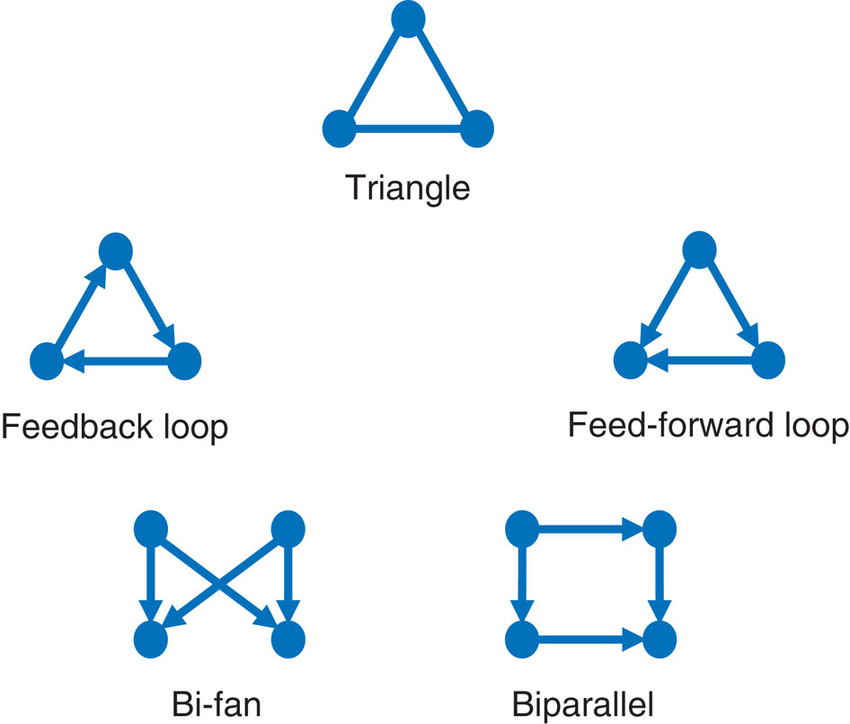
\includegraphics[width=0.9\textwidth]{images/Network-motifs-found-in-biological-networks-The-feed-forward-loop-bi-fan-and-biparallel.png}
    \caption[Network motifs in directed and undirected networks]{Network motifs in directed and undirected networks. In an undirected network the feedback and feed-forward loop would be identical (the triangle at the top of the image. Image from \cite{ngoc2013counting} Attribution-NonCommercial-ShareAlike 3.0 Unported (CC BY-NC-SA 3.0)}
    \label{fig:motifs}
\end{figure}

 TopoGSA \cite{glaab2010topogsa} for a given gene set calculates network parameters such as degree, local clustering coefficient, shortest path length, node betweenness and eigenvector centrality along with a Fisher's exact test for pathways which work contains genes in the set in KEGG, Interpr, BioCarta or Gene Ontology and with network data provided by querying the STRING database\cite{szklarczyk2019string}. An overall similarity score is provided based on the sum of ranks. For an explanation of network metrics see chapter~\ref{chap:Centrality measures}.

It has an easy to use web interface but the user must decide on a cut off significance level and no use is made of the ranks of the genes in the set. 

% The use of network statistics at an individual level for cognitive abilities show no correlation with gene $p$ value for the CAGES data set \footnote{nor for the later datasets}.
The authors do not record if they use direct interactions, or interactions based on techniques such as literature data mining, which are available in STRING\footnote{search tool for recurring instances of neighbouring genes - originally a genomic context database}\cite{szklarczyk2019string}. Finally the web based interface makes it impractical for large scale analysis of GWAS data. 
% It is essentially a, a tool for exploratory gene expression analysis and it is not clear that it has an advantage over GSEA using the BROAD institute's MSigDB database \cite{liberzon2015molecular}. 

The Enrichnet package (2012) by the same author \cite{glaab2012enrichnet} makes greater use of network topology, calculating a distance metric between the gene sets and the STRING database, using a random walk with restart (Xd distance). This is compared to the result of Fisher's exact test. Again the approach identifies pathways by a re-weighting of Fisher's exact test using network topology. I found it hard to interpret the significance of its results and would not be able to use it to test a hypothesis about the synaptic proteome.

It is relatively widely used with 87 citations \footnote{check}. The use of random walk to make a sample of a particular network incorporate information about link density similar to community structure. 

H Nguyen et al. \cite{nguyen2019comprehensive} provide a comprehensive survey of identification of active subnetwork modules. The authors discuss topological modules citing Girvan and Newman (2002) \cite{girvan2002community} and their initial description is similar to modularity defined communities. Most of the methods however seek to find a group of genes closely related in the network to a set of differentially expressed genes (an induced sub graph). Of the 22 methods reviewed only DIAMOnD \cite{ghiassian2015disease} and Enrichnet \cite{glaab2012enrichnet} are not constrained to use differential expression levels of genes in gene expression studies. The method I will describe is designed for the secondary analysis of GWA studies but can easily be adapted to look at differentially expressed genes (see discussion ~\ref{sec:discussion using our method on gene expression}) but the converse is not true. The majority of these approaches try to find an induced subgraph of the network which optimises a cost or utility function based on gene expression or association with disease. The approach in this thesis is to find structures based on network theory and test if they are associated with a specific phenotype. I discuss this further in the discussion section~\ref{sec:discussion more discussion of previous approaches}. 
% Inputs are typically lists of differential expression (p8.25.7) or fold changes rather than a standard summary of GWA data.

% The majority also use directed graphs which allow the identification of motifs more easily or pathway equivalence but are generally not used in protein-protein interactions graphs but rather in metabolic pathways such as KEGG. 
\subsubsection{General points from these reviews}
Mitrea\cite{mitrea2013methods} and Nguyen \cite{nguyen2018network} draw attention to the fact that the results of methods that actually use network topology are difficult to assess and compare (see the discussion above of Enrichnet). The review points out that it is often impossible to reproduce results even with the cooperation of the authors. A large number of the packages are web based and inflexible in the networks that they use.
\subsubsection{Other approaches}



ToppGene  \cite{chen2009toppgene} provides a guilt by association network function (ToppGenNet).  A set of seed genes is drawn and a test set generated using measures of network centrality: Page rank, Hits with priors and k-step markov prioritisation from a neighbourhood distance selected by the user \cite{chen2009disease}. The advantage is it actually uses recognised network methods and a PPI database (although based on literature and primary proteomics (BIND, BioGRID and HPRD)). The disadvantage is that when the prioritised genes are tested by seeing if they have similar ontology, disease or other term enrichment to the disease (seed) genes. Its guilt by association approach means that for a PPI network such as the synapse there are a lot of associates  and the analysis therefore reduces to the subsequent ORA. A random walk will also be affected by  community structure as the walk will spend longer in communities. This is also the case with the enrichnet package\cite{glaab2012enrichnet}.   
WebGestalt \cite{liao2019webgestalt} also offer network based analysis but consists of over representation of portions of a variety of networks including PPI.




\todo[inline]{just do what you said you would do to Douglas. Do your best and be accurate but point out there may be other bits. bit below moved to discussion label sec:other network gsa intro discussion}





\subsubsection{Other approaches}
\label{sec:intro other approaches}
% Mitrea et al. (2013a), reviewing topology based methods, notes that several techniques that claim to be third generation methods use the pathway topology to provide what is essentially a gene set (ie a pathway or portion there of from KEGG or a similar database) and so exclude information on pathway structure topology. Mitra \cite{mitra2013integrative} et al (2013a) criticised Khatri  et al (2012) for including methods including functional analysis and annotation with Gen
Barabasi \cite{barabasi2011network} reviewed a number of methods that used network based statistics such as clustering coefficient to augment the analysis of gene expression and GWAS studies. Of particular interest is the use of a `disease community' which I will return to in chapter~\ref{chap:community detection}. The difference with these approaches is they are based on heterogeneous lists of disease (see section~\ref{sec:biomedical significance of centrality measures} and \ref{sec:assessment of communities})) 

Pandey et al. report using eigenvector centrality of SNPs within a pathway to prioritise genes for pathway enrichment\cite{pandey2012epistasis}. The edges within the network however refer to gene - gene interaction strength rather than network topology. 

It is interesting to note that Mooney and Wilmot \cite{mooney2015gene} suggest using gene sets derived from network analyses. In the course of describing the DiaMOND algorithm Ghiassian et al.\cite{ghiassian2015disease} report comparing topological communities generated using the Louvain \cite{blondel2008fast} (section~\ref{sec:Louvain} and Markov Clustering method \cite{van2000graph} (section~\ref{sec:markov clustering} to a list of disease genes. They concluded that this approach was not useful and hence proposed the DIAMOnD, algorithm. They do not use a tissue specific network and use a variety of definitions of disease genes but do include GWA data from the GWA catalog \cite{macarthur2017new} but use them as items in an over-representation analysis. It is the most similar approach in the literature to the methods in this thesis that I am aware of.
%(Davies et al 2010)
%\footnote{perhaps I should mention WGCNA}.

% Frost et al (2014) describes a spectral method

% for gene set enrichment but this refers to the principle component analysis of a snp matrix and a matrix of indicator variables referring to gene properties.

\section{Plan}
\label{sec:intro plan to procede to next chapter}

I propose an alternative approach would be to use Gene Set Analysis tools widely used in GWA studies and to use as sets the communities identified by a community detection algorithm. In addition I will test the hypothesis that central genes in the network have a central role in cognitive phenotypes. 

To allow the use of a discovery and replication cohort study design in some subsequent sections of this thesis we obtained summary genetic data from meta-analyses  of intelligence and educational attainment to produce discovery and replication samples for each phenotype. The next chapter describes the processing of the data to create the discovery and replication samples and the generation of the interaction graph.








\section{Further discussion}
Lack of different intelligence phenotypes e.g. fluid etc in large scale genomic studies compared with Hill et al. where the finding was for a single phenotype


How findings of GWAS extend to more rare diseases give example of drug induced psychosis or high intelligence

\subsubsection{bits moved to the discussion}
Plomin (new) \cite{plomin2018new} box 5 makes the point about the availability of summary statistics and the non availability of some from commercial enterprises an observation which I completely agree with maybe should move to discussion.
\subsubsection{to discussion}
\label{sec:other network gsa intro discussion}


 
 




